\documentclass{article}

% Course report: show the student name. Remove `final` only if the course
% explicitly requires an anonymous submission.
\usepackage[final]{neurips_2026}

\usepackage[utf8]{inputenc}
\usepackage[T1]{fontenc}
\usepackage{hyperref}
\usepackage{url}
\usepackage{booktabs}
\usepackage{amsmath,amsfonts}
\usepackage{nicefrac}
\usepackage{microtype}
\usepackage{xcolor}
\usepackage{graphicx}
\usepackage{array}
\usepackage{multirow}

\definecolor{instructionblue}{RGB}{20,72,130}
\newcommand{\instruction}[1]{%
  \par\noindent{\color{instructionblue}\small\textbf{[Instruction:} #1\textbf{]}}\par
}
\newcommand{\pp}{\,pp}

\title{[Replace with a title connecting inductive bias, domain shift, generalization, and open-set recognition]}

\author{%
  [Student name]\\
  [Student identifier]\\
  [Course and institution]\\
  \texttt{[student email]}
}

\begin{document}
\maketitle

\begin{abstract}
\instruction{Write one 120--180 word paragraph. State that the report studies behavior beyond IID evaluation; name controlled interventions, unsupervised domain adaptation, domain generalization, and open-set recognition; summarize the strongest Task 1 result; state that mild MMD and SAM worked while excessive MMD collapsed; state that Near unknowns were harder and PROSER was unstable; end with the role of leakage-safe validation and optimization stability. Write this last.}
\end{abstract}

% PAGE BUDGET FOR THE FINAL VERSION:
% title + abstract + introduction: 1.0 page
% Task 1: 2.5 pages
% Task 2: 2.2 pages
% Task 3: 2.0 pages
% Task 4: 2.3 pages
% cross-task discussion: 0.8 page
% deviations/reproducibility: 0.5 page
% conclusion: 0.4 page
% safety margin: 0.3 page

\section{Introduction}

\instruction{Target length: about 0.6 page after the abstract. Explain why IID accuracy can hide reliance on color, texture, position, source-domain artifacts, and closed-set assumptions.}

\instruction{Introduce four questions: how CNN, ViT, and CLIP representations respond to controlled interventions; whether unlabeled target data helps PACS Sketch; whether a model generalizes to Sketch without seeing it; and whether a CIFAR-10 classifier detects semantically Near and Far unknowns.}

\instruction{Give one short contribution sentence per task. Mention seed 6304, fixed splits, validation-only model selection, and isolation of final target or unknown labels. End with a one-sentence report map.}

\section{Task 1: Inductive biases and representations}

\instruction{Target length: 2.5 pages. Use three compact method paragraphs, Tables~\ref{tab:t1-main} and \ref{tab:t1-cue}, and Figure~\ref{fig:t1-main}. Refer to Appendix~\ref{app:t1} for complete consistencies, cosine similarities, and t-SNE plots.}

\subsection{Objective and protocol}

\instruction{State that frozen ResNet-50, ViT-B/16, and CLIP ViT-B/32 representations are compared. Clarify that CLIP uses both a learned linear head and the fixed zero-shot prompt ``a photo of a \{class\}.'', producing four decision rules from three representations.}

\instruction{Describe STL-10: 4,000 training, 1,000 validation, and a fixed balanced 500-image test subset with 50 examples per class. Mention 224-by-224 RGB resizing before each intervention and model-specific normalization. Backbones were frozen. ResNet features were 2,048-D, ViT class-token features 768-D, and CLIP visual embeddings normalized.}

\instruction{Describe the linear heads: AdamW, learning rate 0.001, weight decay 0.0001, at most 50 epochs, patience 5, and validation-accuracy selection. Selected epochs were 13 for ResNet, 6 for ViT, and 14 for the CLIP head. State the hypotheses about modest color sensitivity, increasing translation sensitivity, global-structure dependence after patch shuffle, and model-dependent shape/texture choices.}

\subsection{Controlled interventions}

\begin{table*}[t]
  \caption{STL-10 accuracy under controlled interventions. Translation is averaged over four directions at 32 pixels. Full consistency and displacement results are in Appendix~\ref{app:t1}.}
  \label{tab:t1-main}
  \centering
  \small
  \begin{tabular}{lccccc}
    \toprule
    Decision rule & Clean (\%) & Grayscale (\%) & Hue $45^\circ$ (\%) & Translate 32 (\%) & Patch shuffle (\%) \\
    \midrule
    ResNet-50 head      & 97.80 & 95.60 & 95.20 & 96.75 & 91.60 \\
    ViT-B/16 head       & 97.40 & 95.60 & 96.40 & 96.45 & 90.00 \\
    CLIP ViT-B/32 head  & \textbf{98.40} & \textbf{97.00} & \textbf{96.40} & \textbf{97.80} & 83.40 \\
    CLIP zero-shot      & 98.00 & \textbf{97.00} & \textbf{96.40} & 96.65 & 83.40 \\
    \bottomrule
  \end{tabular}
\end{table*}

\instruction{Introduce Table~\ref{tab:t1-main} before it appears. Discuss that clean results are saturated; CLIP head is numerically highest; color changes cause only modest drops; all 32-pixel translation accuracies remain above 96\%; and patch shuffle is substantially more damaging. Mention that ResNet loses 6.20 percentage points under patch shuffle, ViT 7.40, CLIP head 15.00, and zero-shot CLIP 14.60. Do not equate patch robustness with shape bias.}

\begin{figure*}[t]
  \centering
  \begin{minipage}[t]{0.59\textwidth}
    \centering
    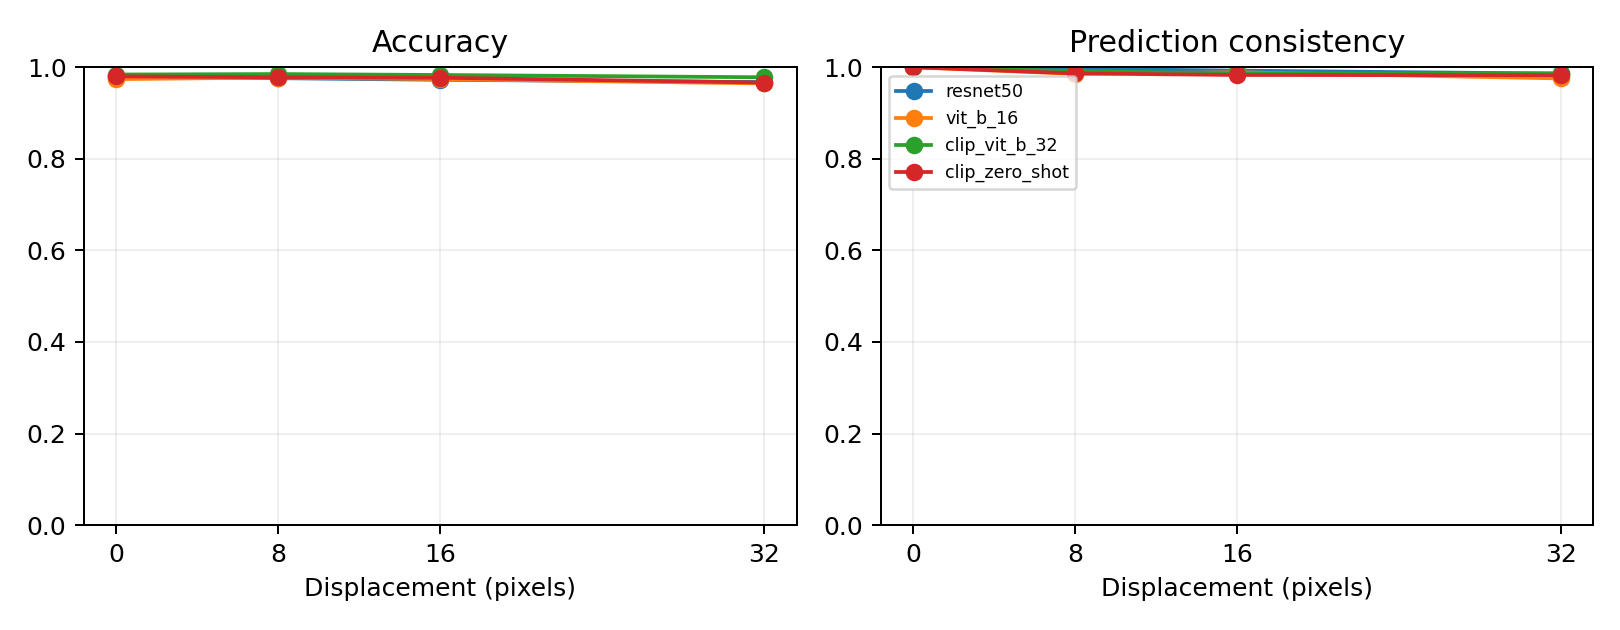
\includegraphics[width=\linewidth]{../task1/results/translation.png}
  \end{minipage}\hfill
  \begin{minipage}[t]{0.38\textwidth}
    \centering
    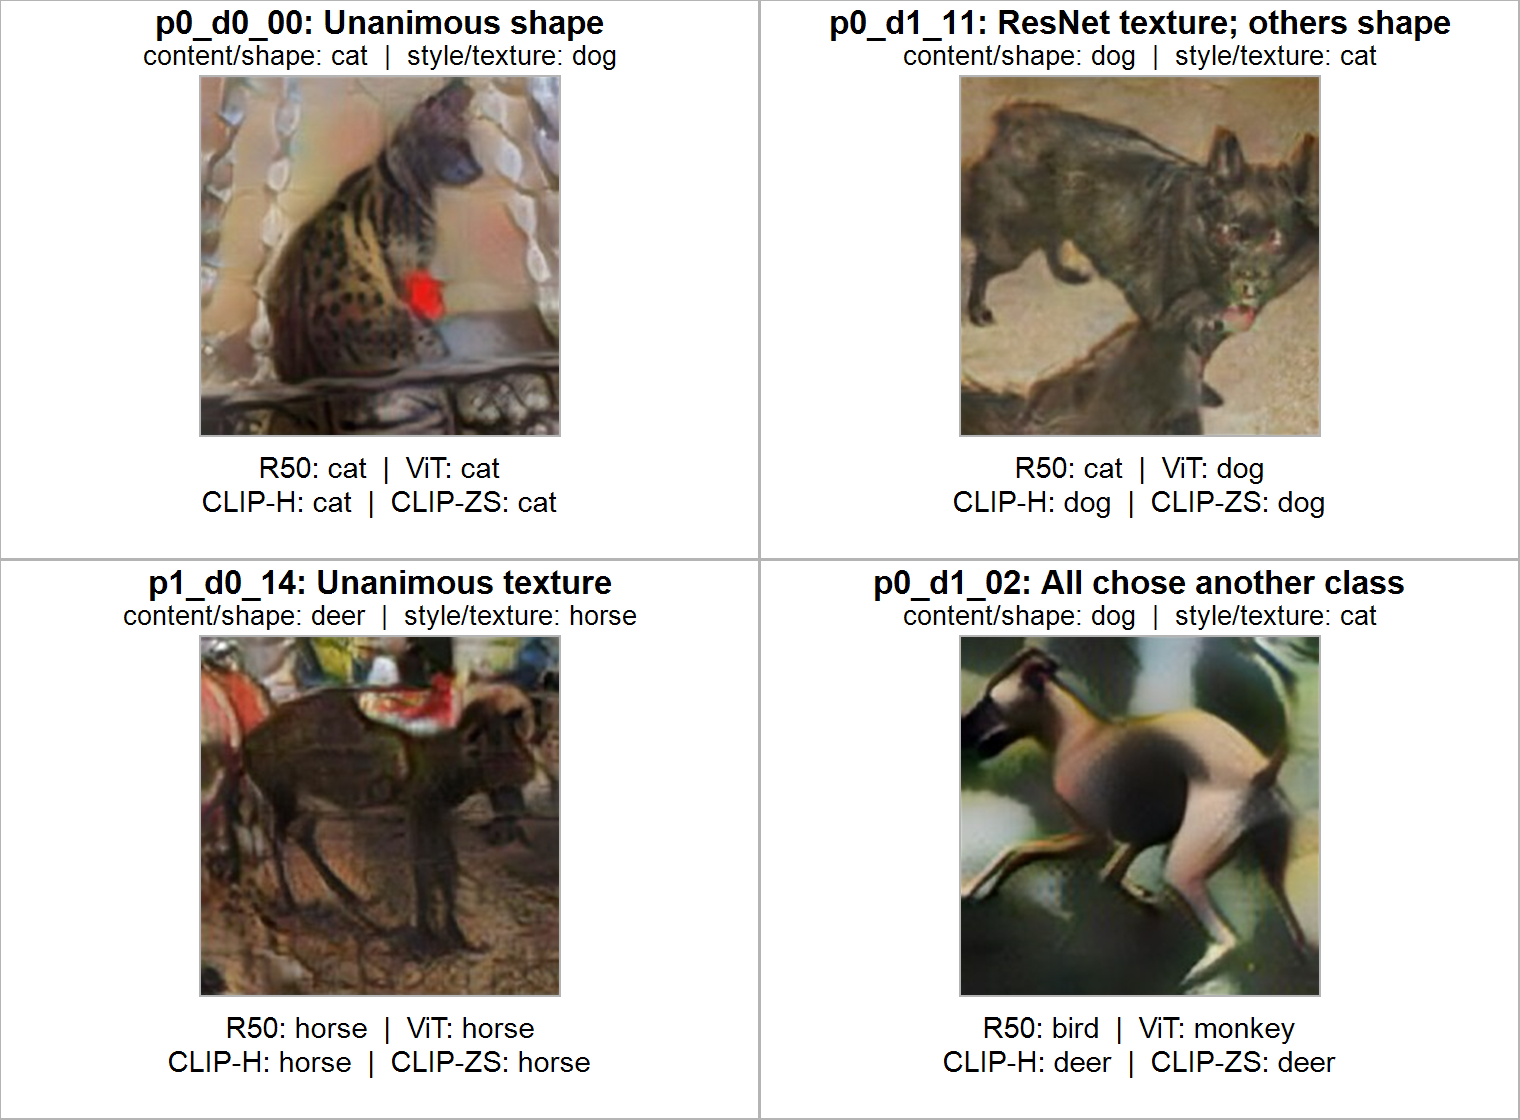
\includegraphics[width=\linewidth]{../task1/results/cue_conflict_examples.png}
  \end{minipage}
  \caption{(a) Mean accuracy and paired prediction consistency over four translation directions, with zero displacement as the clean reference. (b) Reviewed cue-conflict examples annotated with content, style, and predictions. Screening occurred before predictions were viewed.}
  \label{fig:t1-main}
\end{figure*}

\instruction{The cue panel uses p0\_d0\_00 (unanimous shape), p0\_d1\_11 (ResNet texture and the other rules shape), p1\_d0\_14 (unanimous texture), and p0\_d1\_02 (all chose another class). If the combined main figure is unreadable, move the cue panel to Appendix~\ref{app:t1} and retain only the translation image in the main paper.}

\subsection{Cue conflict and representation stability}

\instruction{Describe AdaIN strength 0.8 and five pairs: cat/dog, deer/horse, car/truck, airplane/bird, and airplane/ship, in both directions. Forty candidates per direction produced 400 candidates. Explain the model-blind rejection criteria. Report 348 accepted and 52 rejected: 30 severe artifacts, 17 unrecognizable outlines, 4 both, and 1 severe artifact plus distorted outline. The first 20 accepted images in each of ten groups formed a balanced 200-image set.}

\begin{table}[t]
  \caption{Cue-conflict decisions. Shape bias is shape divided by shape plus texture; coverage is the fraction assigned either cue.}
  \label{tab:t1-cue}
  \centering
  \small
  \begin{tabular}{lrrrrr}
    \toprule
    Model & Shape & Texture & Other & Bias (\%) & Coverage (\%) \\
    \midrule
    ResNet-50 & 144 & 39 & 17 & 78.69 & 91.50 \\
    ViT-B/16 & 171 & 16 & 13 & 91.44 & 93.50 \\
    CLIP head & 172 & 17 & 11 & 91.01 & \textbf{94.50} \\
    CLIP zero-shot & 168 & 14 & 18 & \textbf{92.31} & 91.00 \\
    \bottomrule
  \end{tabular}
\end{table}

\instruction{Discuss Table~\ref{tab:t1-cue}: every rule is shape-oriented, but ViT and CLIP exceed ResNet. Always discuss coverage alongside bias. Mention 120/200 unanimous shape decisions, 24 cases where only ResNet chose texture, and only 3 unanimous texture decisions. Discuss the ResNet airplane/bird direction asymmetry as evidence that bias is pair- and direction-dependent.}

\instruction{Summarize the representation result: translation is most stable, cue conflicts change representations most, and CLIP is generally most stable. Note the mismatch that CLIP has the highest patch cosine similarity but the largest patch-accuracy loss. Refer to Appendix~\ref{app:t1} for exact cosine values and the full t-SNE grid. Limitations: one seed/subset, architecture confounded with pretraining, one CLIP prompt, subjective cue review, AdaIN artifacts, and qualitative t-SNE distortion.}

\section{Task 2: Unsupervised domain adaptation to PACS Sketch}

\instruction{Target length: 2.2 pages. Use one protocol paragraph, one method paragraph, Table~\ref{tab:t2-main}, and Figure~\ref{fig:t2-curves}. Keep original manual runs and supplemental clipped runs visually separated.}

\subsection{Protocol and methods}

\instruction{State the UDA setting: labeled Photo, Art Painting, and Cartoon; unlabeled Sketch during training; Sketch labels used only in final evaluation. Report source train/validation counts in prose: Photo 1,336/334, Art Painting 1,638/410, Cartoon 1,875/469; final Sketch contains 3,929 examples over seven classes. Splits are stratified 80/20 with seed 6304 and selection uses source validation only.}

\instruction{Describe ImageNet-pretrained ResNet-18 with a seven-class head, frozen BatchNorm running statistics, AdamW at $10^{-4}$ learning rate and weight decay, 30 epochs, patience 5, and batches of 8 per source plus 24 unlabeled target images. Explain source-only ERM; DAN with three median-scaled Gaussian MMD kernels and $\lambda\in\{0.1,1,10\}$; DANN with gradient reversal; and CDAN with the feature/probability outer product.}

\instruction{Define source and Sketch accuracy/macro-F1, delta from source-only, per-class accuracy, dominant confusion, and balanced source-target logistic-regression domain probe. State that a low probe score is useful only if class discrimination remains healthy.}

\begin{table*}[t]
  \caption{Task 2 source validation and final PACS Sketch results. Supplemental rows use global gradient clipping with maximum norm 5.}
  \label{tab:t2-main}
  \centering
  \small
  \begin{tabular}{llrrrrr}
    \toprule
    Status & Method & Best epoch & Source F1 & Sketch acc. & Sketch F1 & Probe \\
    \midrule
    \multirow{6}{*}{Original}
      & Source-only & 7 & 0.9334 & 0.5610 & 0.5745 & 0.9959 \\
      & DAN $\lambda=0.1$ & 8 & \textbf{0.9469} & \textbf{0.6872} & \textbf{0.6349} & 0.9657 \\
      & DAN $\lambda=1$ & 1 & 0.0877 & 0.0204 & 0.0057 & 0.6484 \\
      & DAN $\lambda=10$ & 1 & 0.0507 & 0.0407 & 0.0112 & 0.8022 \\
      & DANN & 2 & 0.1276 & 0.0402 & 0.0217 & 0.9986 \\
      & CDAN & 2 & 0.9051 & 0.3489 & 0.4201 & 0.9945 \\
    \midrule
    \multirow{3}{*}{Supplemental}
      & DAN $\lambda=1$ + clip5 & 9 & 0.9331 & 0.6406 & 0.5982 & 0.8214 \\
      & DANN + clip5 & 1 & 0.5929 & 0.0593 & 0.0363 & 0.9986 \\
      & CDAN + clip5 & 11 & 0.9313 & 0.6826 & 0.6277 & 0.9753 \\
    \bottomrule
  \end{tabular}
\end{table*}

\begin{figure*}[t]
  \centering
  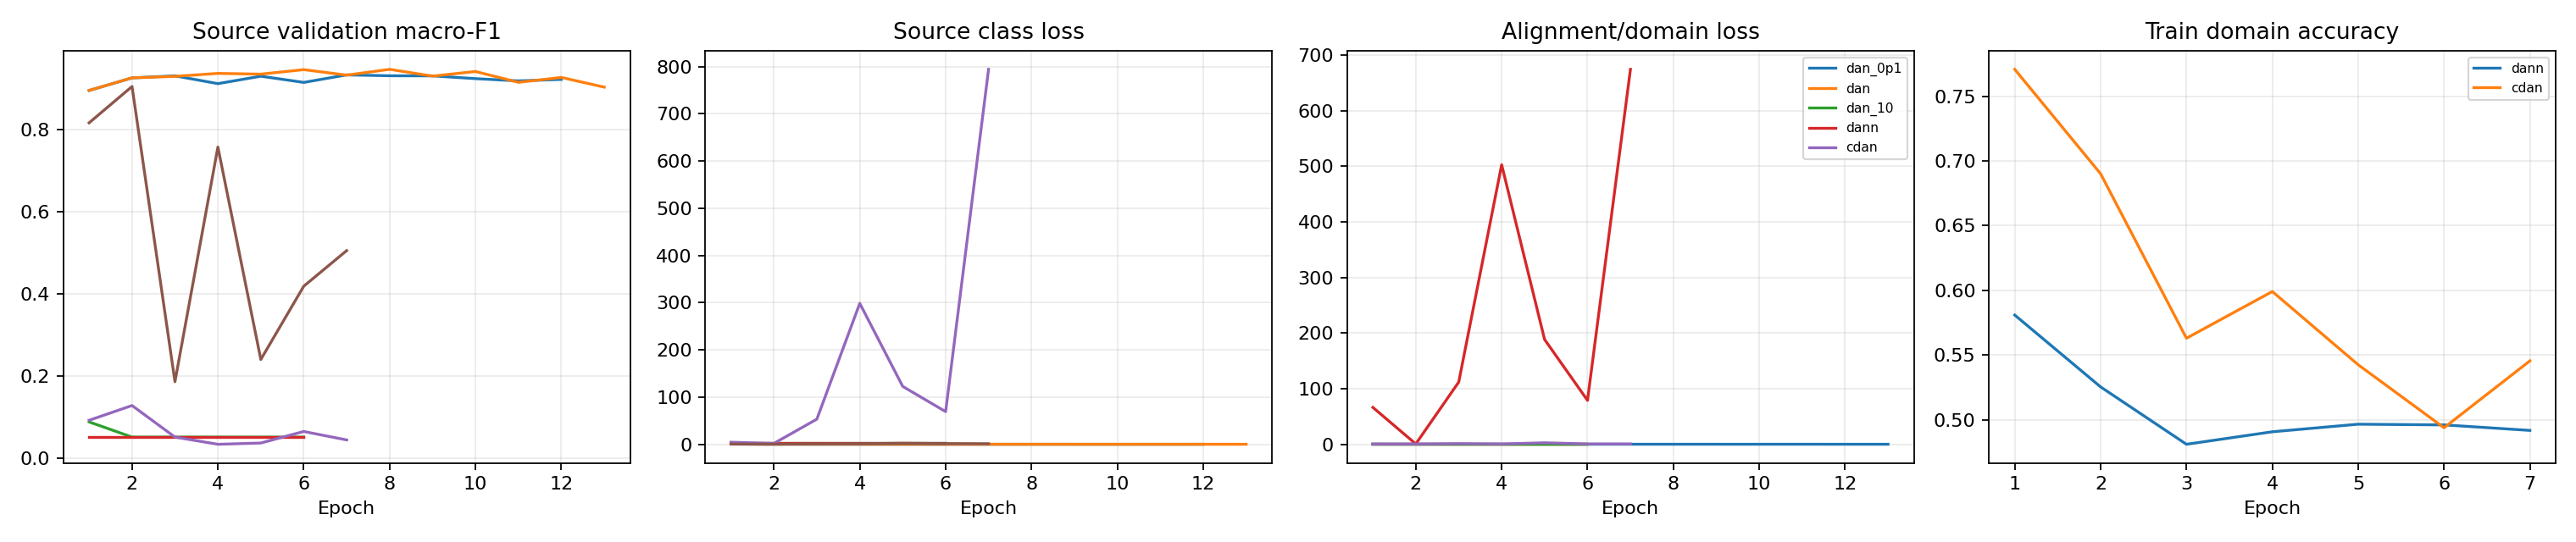
\includegraphics[width=0.98\textwidth]{../task2/results/training_curves.png}\\[3pt]
  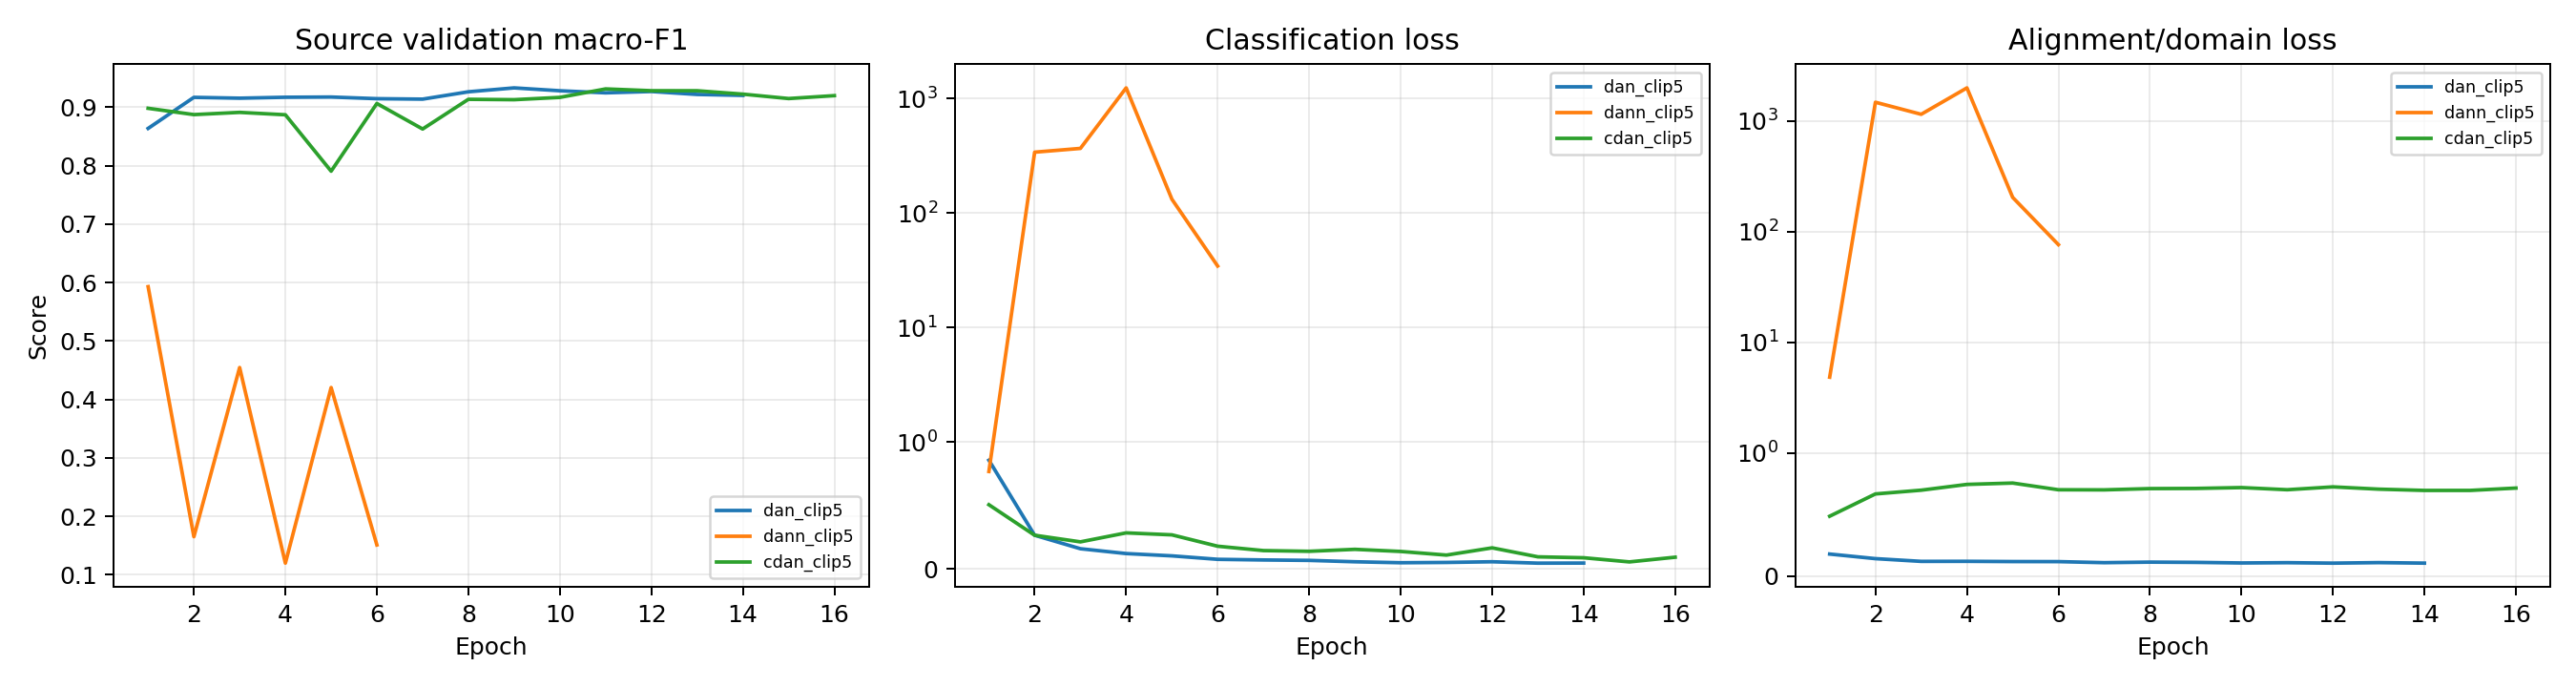
\includegraphics[width=0.90\textwidth]{../task2/supplemental/results/training_curves.png}
  \caption{Original (top) and supplemental clipped (bottom) Task 2 training trajectories. Selection uses source-validation macro-F1. The supplemental loss panels use logarithmic scaling so unstable DANN losses do not hide healthy curves.}
  \label{fig:t2-curves}
\end{figure*}

\subsection{Results and stabilization}

\instruction{Discuss source-only transfer and weak dog, horse, and person classes. DAN 0.1 is the successful manual run: 68.72\% Sketch accuracy, a 12.62-point gain over source-only, while retaining source performance. DAN 1 collapses to house and DAN 10 to person. DANN has exploding losses and poor source/target classification; CDAN is valid at selected epoch 2 but gives negative transfer and later instability. Do not describe collapsed DAN's lower probe score as useful invariance.}

\instruction{Introduce the teaching-assistant-permitted supplemental deviation: after backward and before the optimizer step, clip the global gradient norm at 5. DAN 1 and CDAN recover to 64.06\% and 68.26\% Sketch accuracy; DANN remains failed at 5.93\%. State that DANN's pre-clipping gradient norm reaches 362,803. Conclude that clipping repairs some optimization failures but not all adversarial instability.}

\instruction{Limitations: one seed, backbone, and target direction; a linear probe; imperfect source-only selection; and post-failure supplemental changes that must not replace the original manual results. Refer to Appendix~\ref{app:t2} for counts, per-class results, confusions, and complete curves.}

\section{Task 3: Domain generalization to unseen Sketch}

\instruction{Target length: 2.0 pages. Use Table~\ref{tab:t3-main}; keep complete curves and the fallback sequence in Appendix~\ref{app:t3}.}

\subsection{Protocol and methods}

\instruction{Contrast Task 3 with Task 2: Photo, Art Painting, and Cartoon are available, while no Sketch image or label is used for training, diagnostics, selection, or fallback decisions. The Task 2 split and source-only checkpoint were reused and verified by SHA-256.}

\instruction{Explain DAN-DG as the mean MMD over Photo--Art, Photo--Cartoon, and Art--Cartoon feature pairs for $\lambda\in\{0.1,1,10\}$. Explain nonadaptive two-pass SAM with radius 0.05. Define mean/worst source F1, Sketch metrics, balanced three-way source-domain separability with chance $1/3$, and the fixed-radius sharpness proxy. Warn that low separability or sharpness is meaningless after class collapse.}

\begin{table*}[t]
  \caption{Task 3 source and unseen-Sketch results. The final row is a disclosed supplemental variant using feature-normalized MMD and clipping.}
  \label{tab:t3-main}
  \centering
  \scriptsize
  \begin{tabular}{llrrrrrrr}
    \toprule
    Status & Method & Epoch & Source F1 & Worst F1 & Sketch acc. & Sketch F1 & Separability & Sharpness \\
    \midrule
    \multirow{5}{*}{Original}
      & ERM & 7 & 0.9334 & 0.8995 & 0.5610 & 0.5745 & 0.8638 & 0.3340 \\
      & DAN-DG 0.1 & 9 & 0.9529 & 0.9249 & \textbf{0.7109} & 0.7199 & 0.7907 & 0.1180 \\
      & DAN-DG 1 & 1 & 0.0507 & 0.0421 & 0.0407 & 0.0112 & 0.5847 & 0.0103 \\
      & DAN-DG 10 & 1 & 0.0507 & 0.0421 & 0.0407 & 0.0112 & 0.5415 & 0.0112 \\
      & SAM & 8 & \textbf{0.9567} & \textbf{0.9394} & 0.7045 & \textbf{0.7466} & 0.8638 & \textbf{0.1117} \\
    \midrule
    Supplemental & DAN-DG 1 norm + clip5 & 3 & 0.9284 & 0.8959 & 0.6261 & 0.6321 & 0.6611 & 46.9051 \\
    \bottomrule
  \end{tabular}
\end{table*}

\subsection{Results and stabilization}

\instruction{Discuss DAN-DG 0.1: a 14.99-point gain over ERM and lower, still healthy source-domain separability. Discuss SAM: slightly lower accuracy than DAN-DG 0.1 but the highest macro-F1 and worst-source F1, with meaningful sharpness reduction. DAN-DG 1/10 predict person for every Sketch image; class loss is near $\log 7$, so low sharpness reflects a constant unusable solution.}

\instruction{Compare Tasks 2 and 3 briefly: ERM 56.10/57.45 accuracy/F1, Task 2 DAN 0.1 68.72/63.49, Task 3 DAN-DG 0.1 71.09/71.99, and SAM 70.45/74.66. State that target-free methods are competitive in this run, without claiming that DG generally outperforms UDA.}

\instruction{Document the staged supplemental choice: clip5 alone failed the source-only gate; then each 512-D feature was L2-normalized before MMD while $\lambda=1$ and clipping were retained. This recovers 62.61\% accuracy, 6.52 points above ERM, but remains below DAN-DG 0.1 and SAM. Its sharpness is 46.9051 and it deteriorates after selected epoch 3, so do not call it flat or fully stable. Feature normalization changes the objective and must remain labeled supplemental.}

\instruction{Limitations: one unseen domain, seed, and backbone; linear separability; one-batch one-direction sharpness; imperfect source selection; and post-failure stabilization. Refer to Appendix~\ref{app:t3} for complete curves and diagnostics.}

\section{Task 4: Open-set recognition}

\instruction{Target length: 2.3 pages. Use Tables~\ref{tab:t4-scores} and \ref{tab:t4-models} plus Figure~\ref{fig:t4-main}. Put full metrics, training trajectories, and PROSER dummy diagnostics in Appendix~\ref{app:t4}.}

\subsection{Protocol, models, and scores}

\instruction{Explain closed-set classification versus unknown detection. CIFAR-10 was split into 45,000 train, 5,000 validation, and 10,000 test images. CIFAR-100 was opened only after checkpoints were frozen. Near and Far subsets contain 800 examples each. List Near classes: bus, pickup truck, motorcycle, tractor, wolf, fox, leopard, camel. List Far classes: bottle, bowl, chair, clock, keyboard, mushroom, sunflower, wardrobe.}

\instruction{Describe the CIFAR ResNet-18 stem. Vanilla uses SGD, learning rate 0.1, momentum 0.9, weight decay $5\times10^{-4}$, cosine decay, 100 epochs, crop/flip. GCSC adds RandAugment(2,9). PROSER starts from selected Vanilla, adds five dummy classifiers, and fine-tunes the full network for 50 epochs at learning rate 0.001, $\beta=1$, $\gamma=0.1$, manifold-mixup $\alpha=2$.}

\instruction{Define MSP unknownness $1-\max p$, MLS unknownness $-\max z$, Energy $-\log\sum_c e^{z_c}$, minimum diagonal shared-covariance Mahalanobis distance, and PROSER's strongest-dummy relative to strongest-known score. Each threshold is the 95th percentile of the corresponding CIFAR-10 validation score. Define AUROC, known acceptance, and unknown rejection.}

\begin{table}[t]
  \caption{Vanilla open-set scores. Near and Far denote the selected CIFAR-100 semantic groups; known acceptance and unknown rejection use validation-only thresholds.}
  \label{tab:t4-scores}
  \centering
  \scriptsize
  \begin{tabular}{lrrrrrr}
    \toprule
    Score & Near AUC & Far AUC & All AUC & Known accept. & Near rej. & Far rej. \\
    \midrule
    MSP & \textbf{0.8265} & 0.9061 & \textbf{0.8663} & 0.9500 & 0.2900 & 0.4638 \\
    MLS & 0.8117 & 0.9075 & 0.8596 & 0.9466 & 0.3563 & 0.5775 \\
    Energy & 0.8117 & 0.9081 & 0.8599 & 0.9444 & \textbf{0.3663} & \textbf{0.5875} \\
    Mahalanobis & 0.8007 & \textbf{0.9201} & 0.8604 & 0.9523 & 0.2675 & 0.5275 \\
    \bottomrule
  \end{tabular}
\end{table}

\begin{table}[t]
  \caption{Open-set comparison of trained models and scores at validation-selected operating points.}
  \label{tab:t4-models}
  \centering
  \scriptsize
  \begin{tabular}{lrrrrrr}
    \toprule
    Model/score & Known acc. & Near AUC & Far AUC & All AUC & Near rej. & Far rej. \\
    \midrule
    Vanilla MLS & 0.9467 & 0.8117 & \textbf{0.9075} & \textbf{0.8596} & \textbf{0.3563} & \textbf{0.5775} \\
    GCSC MLS & \textbf{0.9535} & 0.8076 & 0.9078 & 0.8577 & 0.3300 & 0.5775 \\
    PROSER MLS & 0.9407 & \textbf{0.8117} & 0.8708 & 0.8413 & 0.3125 & 0.4550 \\
    PROSER placeholder & 0.9407 & 0.8067 & 0.8927 & 0.8497 & 0.3138 & 0.5213 \\
    \bottomrule
  \end{tabular}
\end{table}

\begin{figure*}[t]
  \centering
  \begin{minipage}[t]{0.55\textwidth}
    \centering
    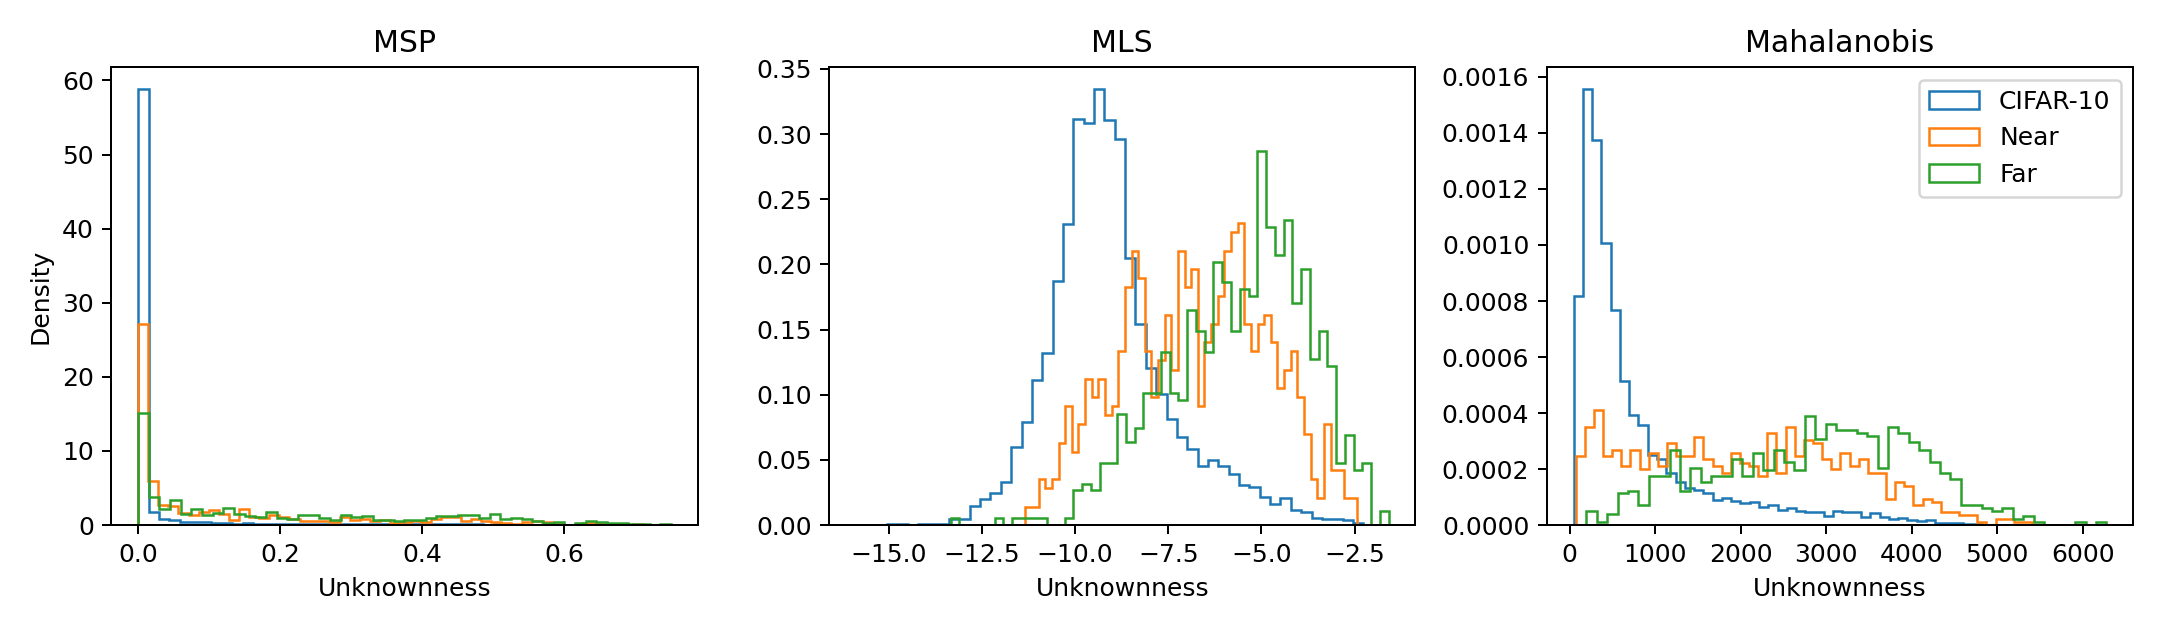
\includegraphics[width=\linewidth]{../task4/results/vanilla_score_distributions.png}
  \end{minipage}\hfill
  \begin{minipage}[t]{0.42\textwidth}
    \centering
    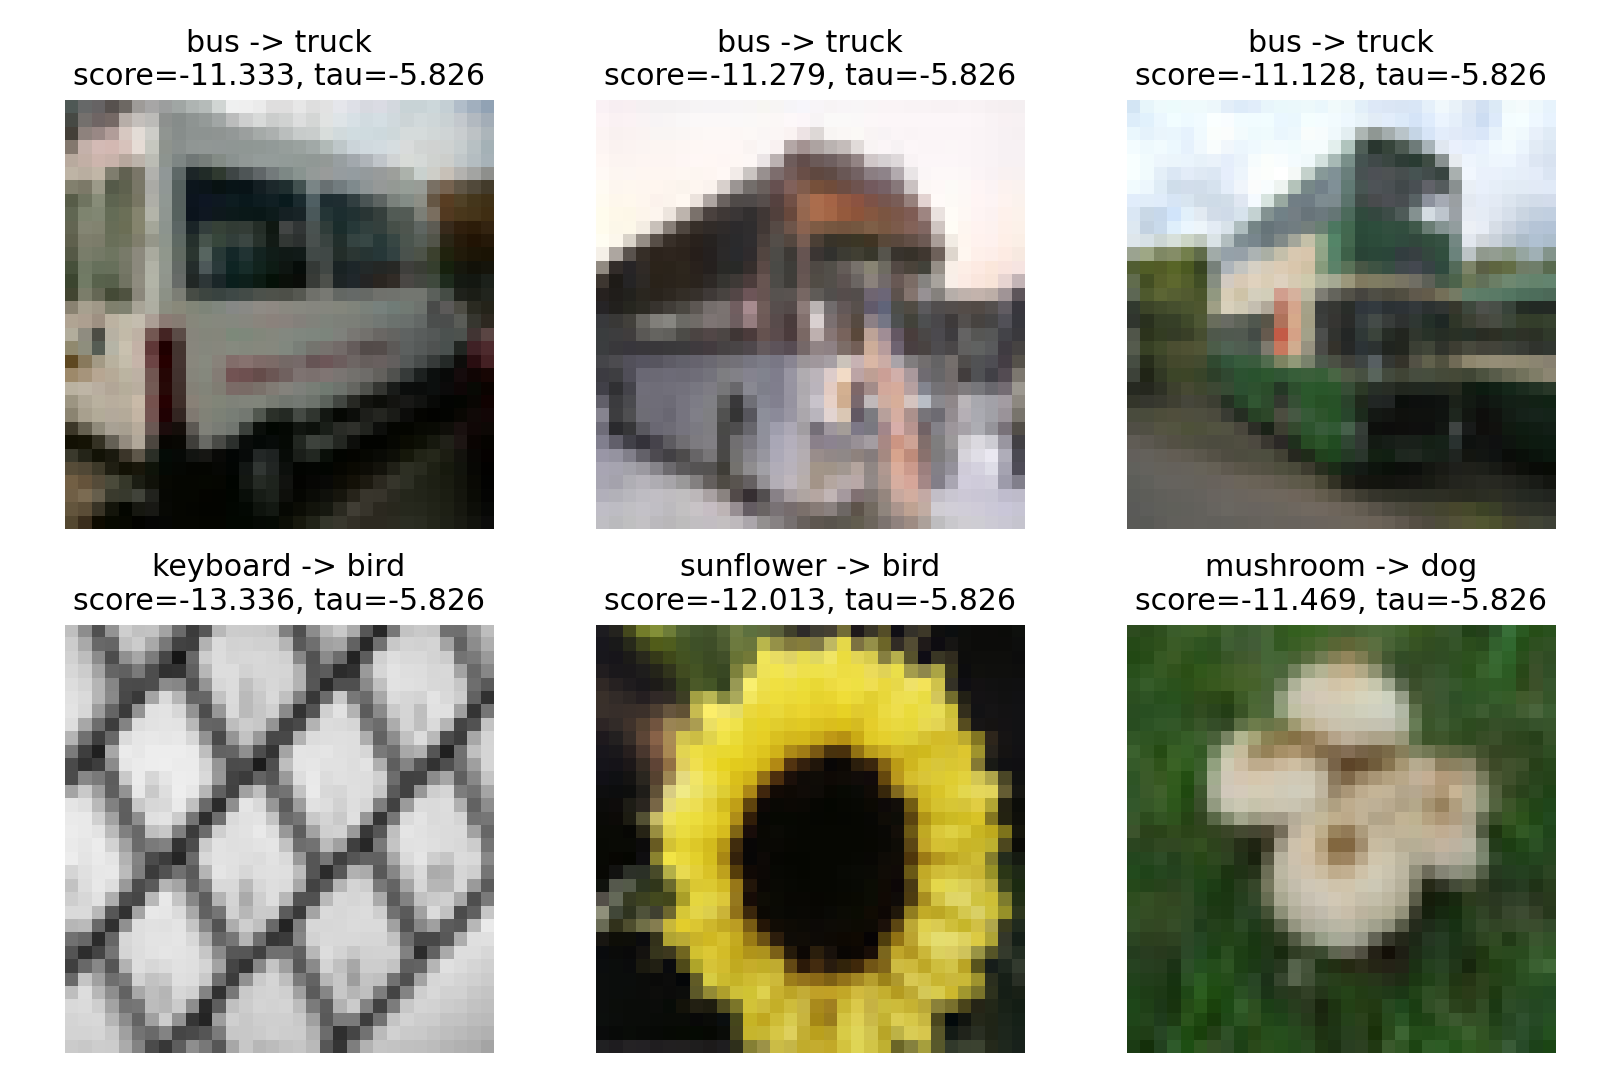
\includegraphics[width=\linewidth]{../task4/results/vanilla_mls_failures.png}
  \end{minipage}
  \caption{(a) CIFAR-10 versus Near/Far unknownness distributions; larger scores mean more unknown. (b) High-confidence Vanilla MLS failures beyond the validation threshold, annotated with predicted CIFAR-10 labels.}
  \label{fig:t4-main}
\end{figure*}

\subsection{Results and failure analysis}

\instruction{Report known performance in prose: Vanilla test accuracy 94.67\%, GCSC 95.35\%, selected PROSER 94.07\%. Explain that GCSC improves known accuracy by 0.68 points without improving overall OSR. Near unknowns are harder. MSP gives the best Near and overall AUROC; Mahalanobis the best Far AUROC; Energy the best thresholded rejection. Rankings depend on metric.}

\instruction{Vanilla MLS is the strongest overall trained-model row. PROSER's placeholder improves its own Far behavior relative to PROSER MLS but remains below Vanilla. State directly that improved closed-set accuracy does not guarantee improved open-set detection.}

\instruction{Discuss failures cautiously: buses predicted as trucks are plausible Near errors due to shared vehicle structure and context; keyboard-to-bird, sunflower-to-bird, and mushroom-to-dog are surprising Far errors that may reflect local texture, silhouette, or background. Do not assert a causal mechanism without attribution evidence.}

\instruction{Document supplemental PROSER clip5. Best validation rises only 0.9438 to 0.9446, epoch-50 validation rises 0.8262 to 0.9040, test accuracy changes 0.9407 to 0.9408, MLS All AUROC 0.8413 to 0.8414, and placeholder All AUROC 0.8497 to 0.8501. Dummy wins are 8.02\% at selected epoch 1, above 81\% by epoch 10, and about 100\% from epoch 22. Clipping improves the late known-class trajectory but barely changes selected-checkpoint OSR.}

\instruction{Limitations: one seed/architecture, fixed unknown class lists, shared CIFAR visual format, one threshold policy, diagonal covariance, qualitative failure explanations, and unstable PROSER optimization.}

\section{Cross-task discussion}

\instruction{Target length: 0.8 page. Synthesize instead of repeating tables. Connect Task 1 controlled changes to Tasks 2--3 domain shift: high clean accuracy does not guarantee stable behavior after structural, style, or domain changes.}

\instruction{Connect Tasks 2 and 3: mild alignment helps, excessive alignment removes class information, and target access does not prevent collapse. Connect SAM and the supplemental runs to the broader point that optimization stability matters, while no single gradient, separability, or sharpness diagnostic is sufficient.}

\instruction{Connect Task 4: higher known accuracy does not ensure unknown detection, paralleling how lower domain separability does not ensure target classification. State the general measurement lesson: pair accuracy with consistency, shape bias with coverage, invariance with class utility, and AUROC with operating-point rejection. Mention validation-only selection and frozen final evaluation.}

\section{Deviations and reproducibility}

\instruction{Target length: 0.5 page. Introduce Table~\ref{tab:deviations}. Mention seed 6304, saved splits, fixed subsets, checkpoint hashes, fixed prompts, model-blind cue review, validation-only thresholds, and isolation of Sketch labels/CIFAR-100 during selection.}

\begin{table*}[t]
  \caption{Supplemental deviations from the manual. Original results were retained and reported separately.}
  \label{tab:deviations}
  \centering
  \small
  \begin{tabular}{llll}
    \toprule
    Change & Tasks & Status & Disclosure \\
    \midrule
    Global gradient clipping, max norm 5 & 2, 3, 4 & Run & Supplemental; outside manual optimizer recipe \\
    L2 feature normalization before MMD & 3 & After clip-only failure & Changes MMD inputs/objective \\
    Gradient/prediction/dummy diagnostics & 2, 3, 4 & Run & Logging only; no optimization change \\
    \bottomrule
  \end{tabular}
\end{table*}

\instruction{State that the teaching assistant permitted stabilization changes when documented with reasoning. Original runs were never silently replaced, and target or unknown labels were unavailable during supplemental selection.}

\section{Conclusion}

\instruction{Target length: one compact paragraph, about 0.4 page. Summarize: similar Task 1 clean performance but different intervention/cue behavior; successful mild alignment and SAM but collapsed excessive alignment; selective benefits from clipping/normalization; harder Near unknowns; and PROSER below Vanilla. End by stating that evaluation beyond IID accuracy requires controlled interventions, leakage-safe protocols, and diagnostics that retain class utility.}

% ==================== 12-PAGE MAIN PAPER ENDS HERE ====================
% If the conclusion crosses page 12, shorten prose/captions or move supporting
% material to the appendix. Do not alter the NeurIPS style file.

\section*{References}

\instruction{Add verified references for STL-10, PACS, CIFAR-10/100, ResNet, ViT, CLIP, AdaIN, DAN/MMD, DANN, CDAN, SAM, GCSC, and PROSER. Use one consistent natbib-compatible style. References do not count toward the main-paper page limit under the supplied NeurIPS template, but confirm the course rule.}

{\small
\begin{enumerate}
  \item \textbf{[Replace with verified STL-10/PACS/CIFAR references.]}
  \item \textbf{[Replace with verified model and method references.]}
  \item \textbf{[Remove this placeholder list after adding the bibliography.]}
\end{enumerate}
}

\clearpage
\appendix

\section{Task 1 supporting results}
\label{app:t1}

\subsection{Data split and complete protocol}
\instruction{Use the split table below while describing preprocessing order, feature dimensions, head optimization, selected epochs, and the fixed CLIP prompt.}

\begin{table}[h]
  \caption{STL-10 split used in Task 1.}
  \centering
  \begin{tabular}{lr}
    \toprule
    Split & Count \\
    \midrule
    Train & 4,000 \\
    Validation & 1,000 \\
    Fixed test subset & 500 (50/class) \\
    \bottomrule
  \end{tabular}
\end{table}

\subsection{Complete intervention results}
\instruction{Discuss these expanded tables only as needed; the main paper already contains their condensed accuracy columns. State that each image used a deterministic, seeded nonidentity 4-by-4 patch permutation.}

\begin{table}[h]
  \caption{Clean STL-10 performance before intervention.}
  \centering
  \small
  \begin{tabular}{lrrr}
    \toprule
    Decision rule & Accuracy (\%) & Macro-F1 (\%) & Mean max confidence \\
    \midrule
    ResNet-50 head & 97.80 & 97.80 & 0.977 \\
    ViT-B/16 head & 97.40 & 97.39 & 0.968 \\
    CLIP ViT-B/32 head & \textbf{98.40} & \textbf{98.40} & 0.850 \\
    CLIP zero-shot & 98.00 & 97.99 & 0.955 \\
    \bottomrule
  \end{tabular}
\end{table}

\instruction{Do not compare confidence as if it were calibrated across these decision rules because their score constructions differ.}

\begin{table*}[h]
  \caption{Complete grayscale and fixed $45^\circ$ hue-rotation results. Delta is relative to clean accuracy.}
  \centering
  \small
  \begin{tabular}{lrrrrrr}
    \toprule
    Model & Gray acc. (\%) & Gray delta & Gray cons. (\%) & Hue acc. (\%) & Hue delta & Hue cons. (\%) \\
    \midrule
    ResNet-50 & 95.60 & $-2.20\pp$ & 96.00 & 95.20 & $-2.60\pp$ & 96.00 \\
    ViT-B/16 & 95.60 & $-1.80\pp$ & 95.60 & 96.40 & $-1.00\pp$ & 97.00 \\
    CLIP head & 97.00 & $-1.40\pp$ & 97.40 & 96.40 & $-2.00\pp$ & 97.20 \\
    CLIP zero-shot & 97.00 & $-1.00\pp$ & 97.20 & 96.40 & $-1.60\pp$ & 97.40 \\
    \bottomrule
  \end{tabular}
\end{table*}

\begin{table}[h]
  \caption{Complete patch-shuffle results.}
  \centering
  \small
  \begin{tabular}{lrrr}
    \toprule
    Model & Accuracy (\%) & Clean delta & Consistency (\%) \\
    \midrule
    ResNet-50 & 91.60 & $-6.20\pp$ & 92.80 \\
    ViT-B/16 & 90.00 & $-7.40\pp$ & 91.20 \\
    CLIP head & 83.40 & $-15.00\pp$ & 84.20 \\
    CLIP zero-shot & 83.40 & $-14.60\pp$ & 83.80 \\
    \bottomrule
  \end{tabular}
\end{table}

\begin{table*}[h]
  \caption{Direction-averaged translation accuracy and paired prediction consistency (percent). Zero pixels is the clean reference.}
  \label{tab:t1-translation-full}
  \centering
  \small
  \begin{tabular}{lrrrrrrrr}
    \toprule
    & \multicolumn{2}{c}{0 px} & \multicolumn{2}{c}{8 px} & \multicolumn{2}{c}{16 px} & \multicolumn{2}{c}{32 px} \\
    \cmidrule(lr){2-3}\cmidrule(lr){4-5}\cmidrule(lr){6-7}\cmidrule(lr){8-9}
    Model & Acc. & Cons. & Acc. & Cons. & Acc. & Cons. & Acc. & Cons. \\
    \midrule
    ResNet-50 & 97.80 & 100.00 & 97.60 & 99.65 & 97.25 & 99.25 & 96.75 & 98.60 \\
    ViT-B/16 & 97.40 & 100.00 & 97.75 & 98.55 & 97.40 & 98.90 & 96.45 & 97.55 \\
    CLIP head & 98.40 & 100.00 & 98.50 & 99.15 & 98.30 & 98.65 & 97.80 & 98.65 \\
    CLIP zero-shot & 98.00 & 100.00 & 97.80 & 98.65 & 97.70 & 98.30 & 96.65 & 98.25 \\
    \bottomrule
  \end{tabular}
\end{table*}

\subsection{Cue review and representation diagnostics}
\instruction{Use Tables~\ref{tab:t1-review} and \ref{tab:t1-cue-pairs} when discussing review balance and pair/direction dependence. The cue-example composite is included below.}

\begin{table}[h]
  \caption{Model-blind cue-candidate review counts by content/style direction.}
  \label{tab:t1-review}
  \centering
  \small
  \begin{tabular}{lrr}
    \toprule
    Content/style & Accepted & Rejected \\
    \midrule
    cat/dog & 31 & 9 \\
    dog/cat & 35 & 5 \\
    deer/horse & 34 & 6 \\
    horse/deer & 36 & 4 \\
    car/truck & 37 & 3 \\
    truck/car & 37 & 3 \\
    airplane/bird & 34 & 6 \\
    bird/airplane & 30 & 10 \\
    airplane/ship & 37 & 3 \\
    ship/airplane & 37 & 3 \\
    \midrule
    Total & 348 & 52 \\
    \bottomrule
  \end{tabular}
\end{table}

\begin{table}[h]
  \caption{Recorded rejection reasons for the 52 excluded cue candidates.}
  \label{tab:t1-rejection-reasons}
  \centering
  \small
  \begin{tabular}{lr}
    \toprule
    Reason & Count \\
    \midrule
    Severe artifacts & 30 \\
    Content outline not recognizable & 17 \\
    Both severe artifacts and unrecognizable outline & 4 \\
    Severe artifacts and distorted outline & 1 \\
    \bottomrule
  \end{tabular}
\end{table}

\begin{table*}[h]
  \caption{Cue decisions by content/style direction. Each cell gives shape/texture/other counts over 20 balanced accepted examples.}
  \label{tab:t1-cue-pairs}
  \centering
  \small
  \begin{tabular}{lrrrr}
    \toprule
    Content/style & ResNet-50 & ViT-B/16 & CLIP head & CLIP zero-shot \\
    \midrule
    cat/dog & 14/0/6 & 17/0/3 & 18/1/1 & 13/3/4 \\
    dog/cat & 14/3/3 & 15/0/5 & 14/2/4 & 15/1/4 \\
    deer/horse & 18/2/0 & 19/1/0 & 17/2/1 & 17/2/1 \\
    horse/deer & 15/5/0 & 18/1/1 & 19/0/1 & 20/0/0 \\
    car/truck & 17/2/1 & 20/0/0 & 19/1/0 & 19/1/0 \\
    truck/car & 17/3/0 & 16/4/0 & 16/3/1 & 16/4/0 \\
    airplane/bird & 0/18/2 & 13/5/2 & 14/5/1 & 13/3/4 \\
    bird/airplane & 17/0/3 & 18/1/1 & 19/0/1 & 17/0/3 \\
    airplane/ship & 13/5/2 & 20/0/0 & 20/0/0 & 19/0/1 \\
    ship/airplane & 19/1/0 & 15/4/1 & 16/3/1 & 19/0/1 \\
    \bottomrule
  \end{tabular}
\end{table*}

\begin{figure}[h]
  \centering
  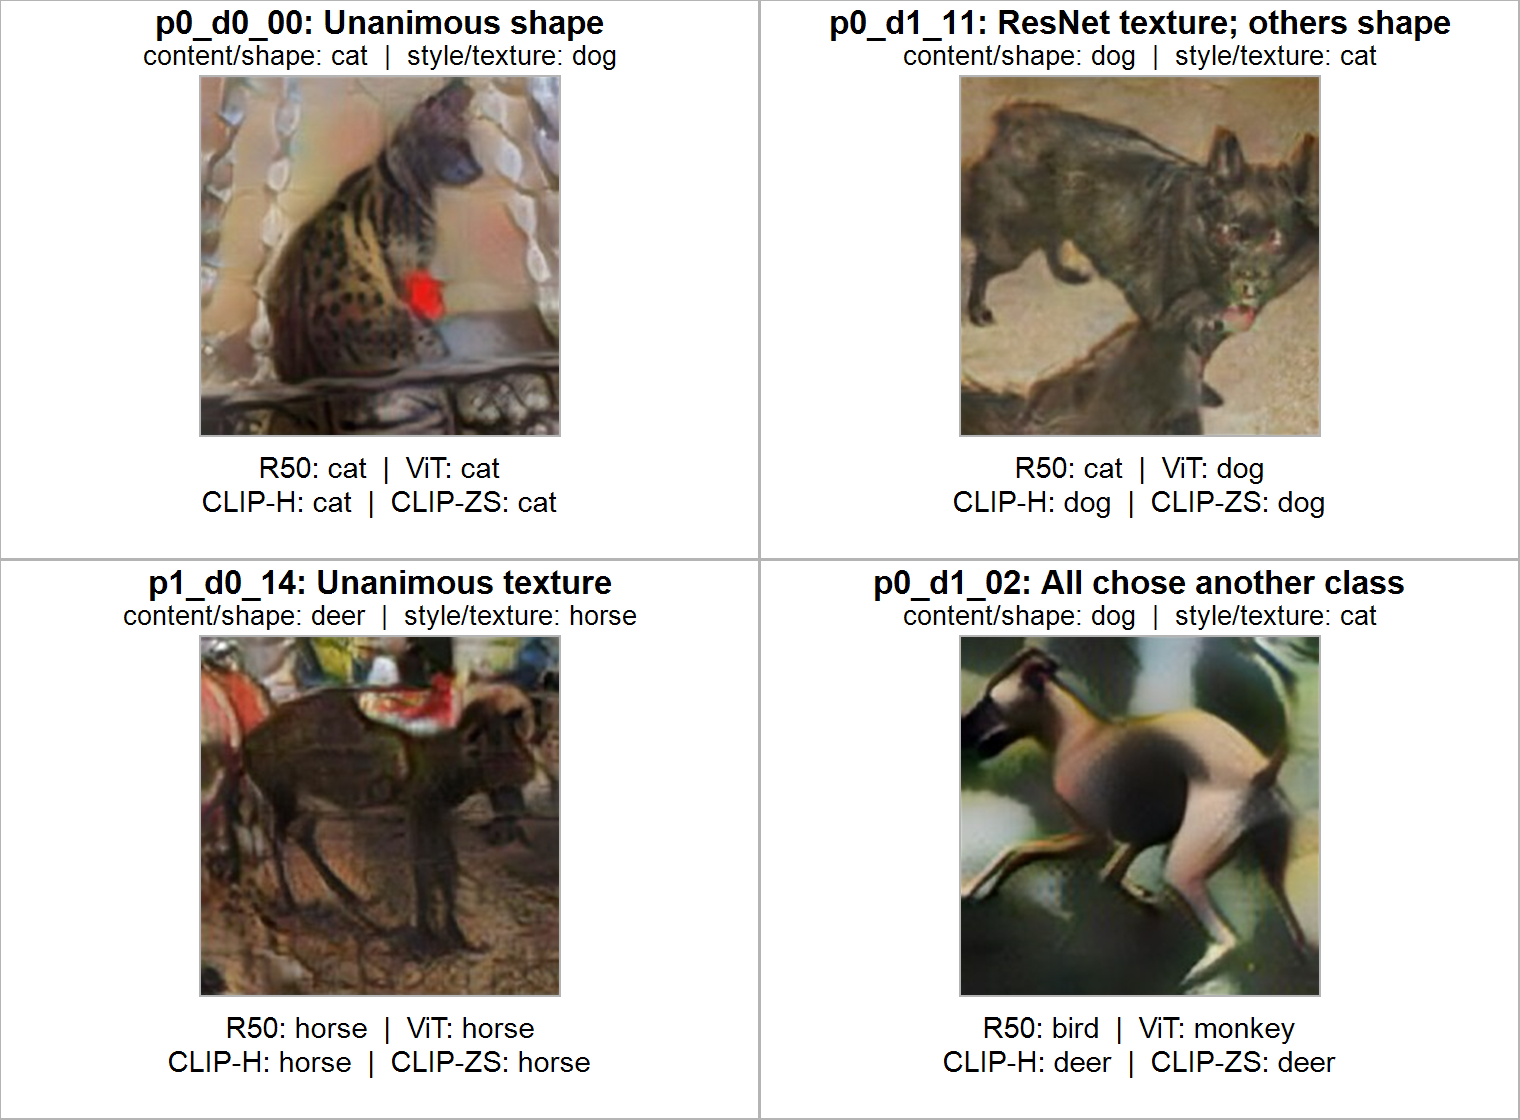
\includegraphics[width=\linewidth]{../task1/results/cue_conflict_examples.png}
  \caption{Reviewed cue-conflict examples spanning unanimous shape, model disagreement, unanimous texture, and predictions outside both intended classes. Content/style labels and all four decision rules are shown in each panel.}
\end{figure}

\begin{table}[h]
  \caption{Mean paired cosine similarity between clean and intervened representations.}
  \centering
  \small
  \begin{tabular}{lrrr}
    \toprule
    Intervention & ResNet-50 & ViT-B/16 & CLIP ViT-B/32 \\
    \midrule
    Grayscale & 0.7884 & 0.7393 & \textbf{0.8983} \\
    Patch shuffle & 0.7180 & 0.6572 & \textbf{0.7281} \\
    Cue conflict & 0.4872 & 0.5213 & \textbf{0.7628} \\
    Translation 8 & 0.9685 & 0.9471 & \textbf{0.9810} \\
    Translation 16 & 0.9525 & \textbf{0.9743} & 0.9680 \\
    Translation 32 & 0.9327 & 0.9418 & \textbf{0.9699} \\
    \bottomrule
  \end{tabular}
\end{table}

\instruction{The composite below has been generated from the twelve saved panels. Use rows ResNet, ViT, CLIP and columns grayscale, patch, cue, translate-32-right when discussing it.}

\begin{figure*}[h]
  \centering
  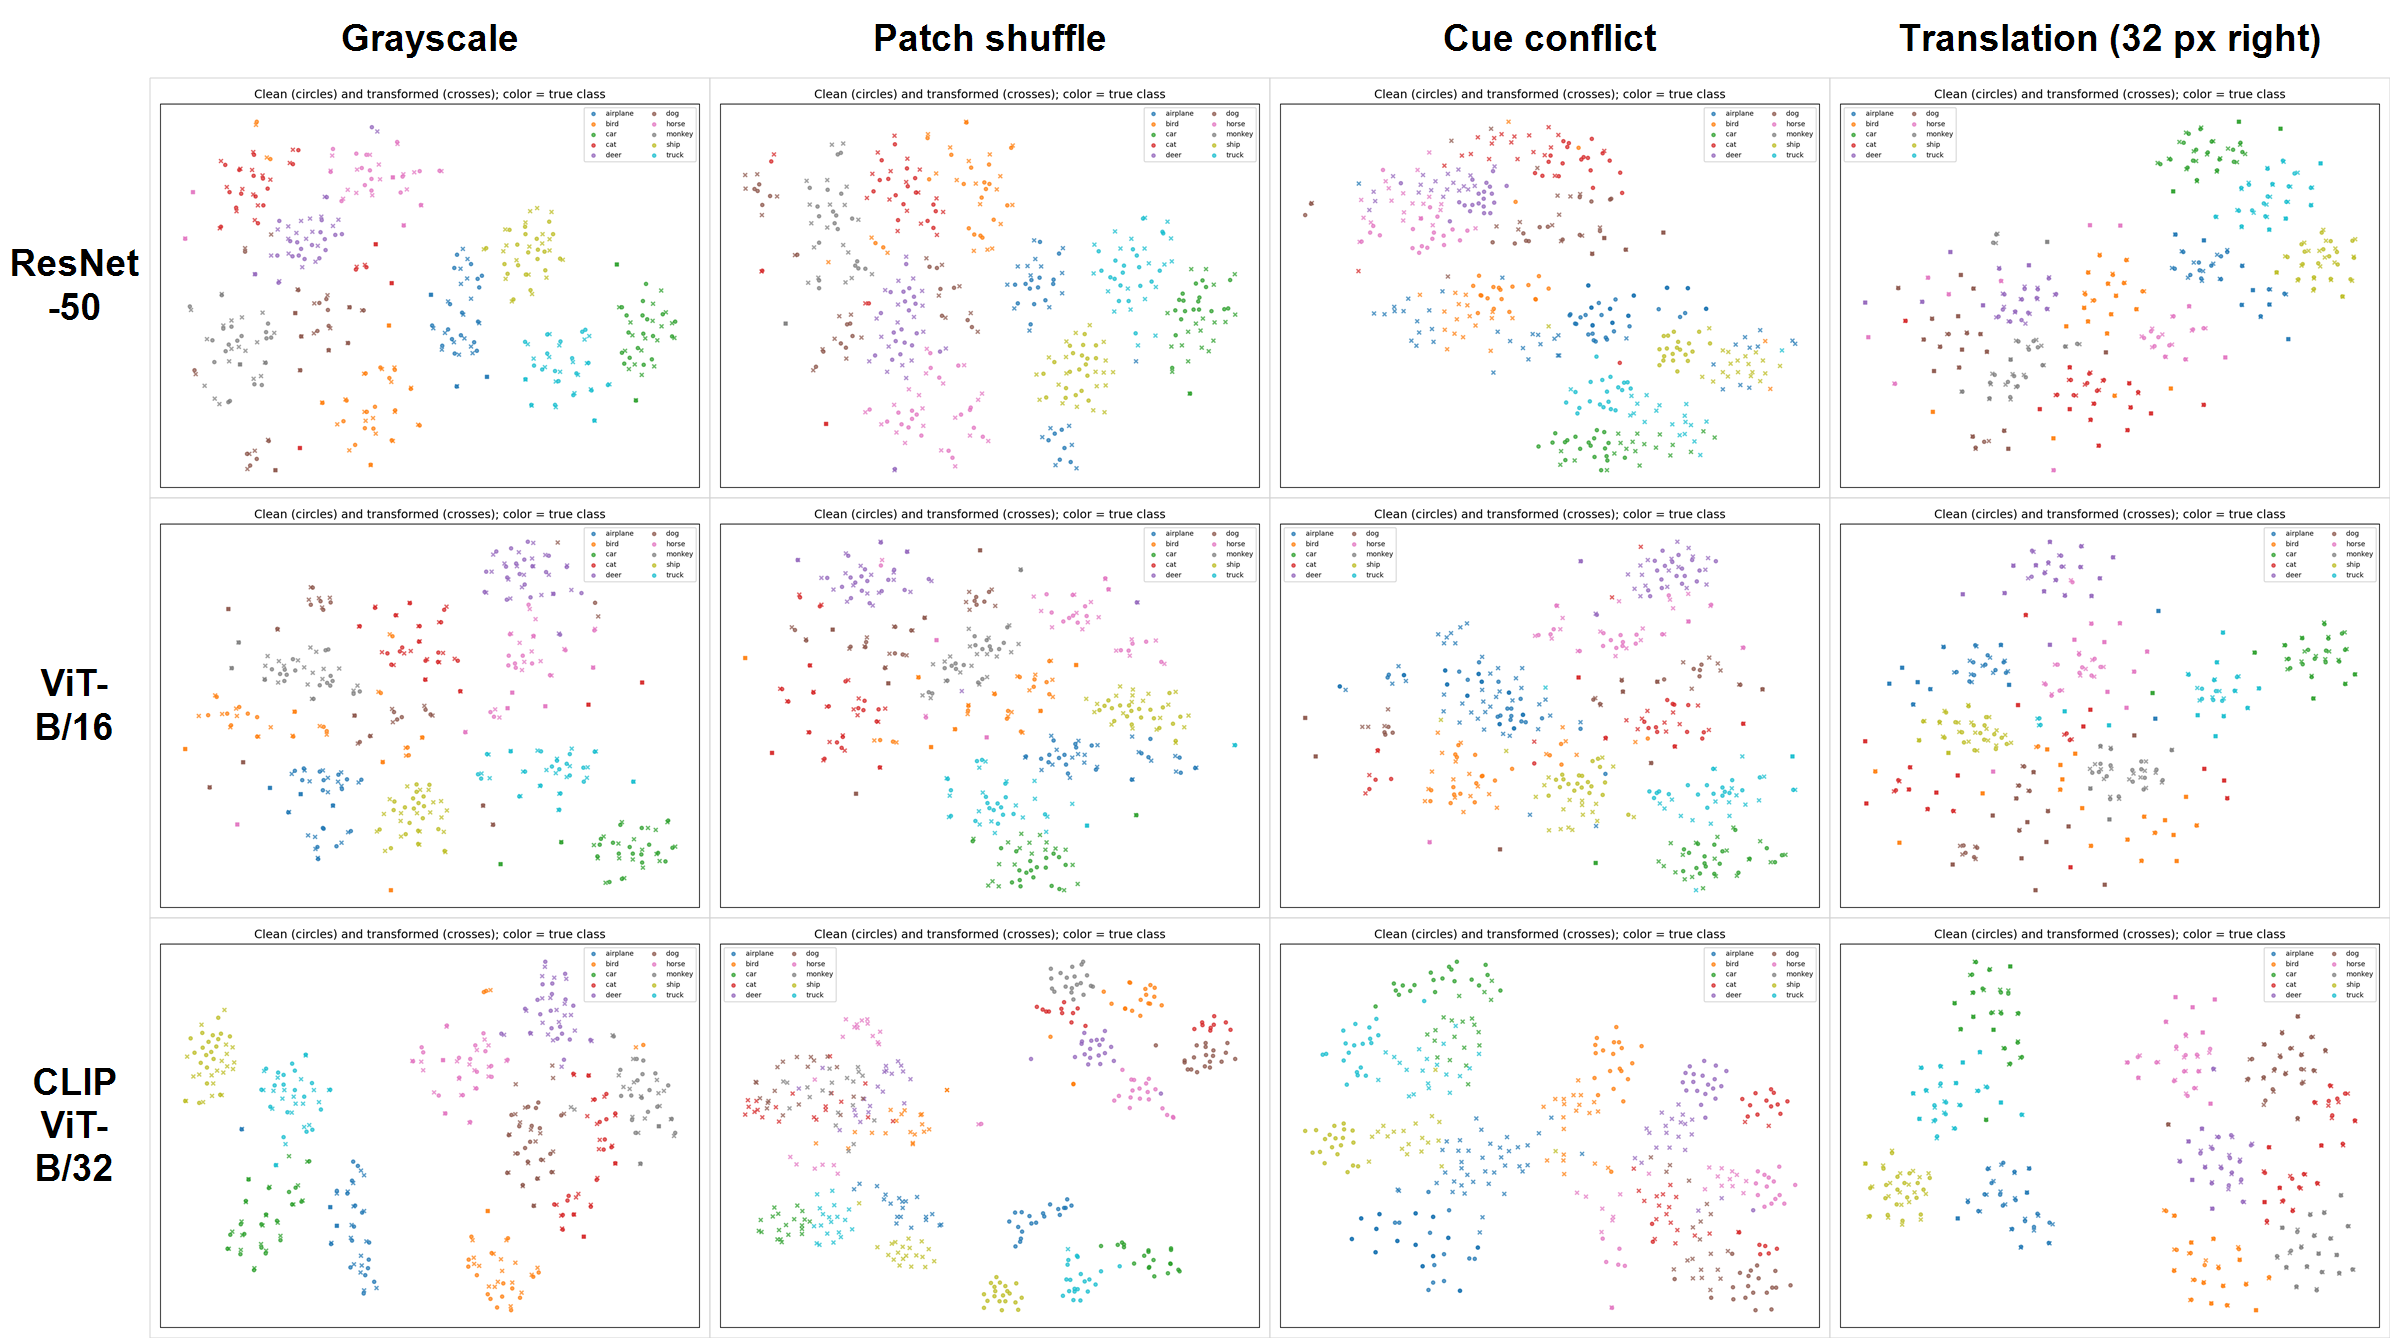
\includegraphics[width=\textwidth]{../task1/results/tsne_grid.png}
  \caption{Joint clean/transformed t-SNE panels. Circles are clean, crosses are transformed, and color is the true class. Each panel was fitted separately, so axes and absolute positions are not comparable across panels.}
\end{figure*}

\clearpage
\section{Task 2 supporting results}
\label{app:t2}

\subsection{PACS counts and complete training protocol}
\instruction{Use Table~\ref{tab:t2-counts} while describing the optimizer and augmentation settings, batch composition, early stopping, and source-only model-selection rule.}

\begin{table}[h]
  \caption{PACS source split and final target size.}
  \label{tab:t2-counts}
  \centering
  \small
  \begin{tabular}{lrr}
    \toprule
    Domain & Train & Validation/final \\
    \midrule
    Photo & 1,336 & 334 \\
    Art Painting & 1,638 & 410 \\
    Cartoon & 1,875 & 469 \\
    Sketch target & Unlabeled & 3,929 final \\
    \bottomrule
  \end{tabular}
\end{table}

\begin{table*}[h]
  \caption{Original Task 2 source-domain validation performance used for model selection.}
  \label{tab:t2-source-domains}
  \centering
  \scriptsize
  \begin{tabular}{lrrrrrrrr}
    \toprule
    Method & Photo acc. & Photo F1 & Art acc. & Art F1 & Cartoon acc. & Cartoon F1 & Mean acc. & Mean F1 \\
    \midrule
    Source-only & 0.9731 & 0.9693 & 0.9073 & 0.8995 & 0.9275 & 0.9314 & 0.9360 & 0.9334 \\
    DAN 0.1 & 0.9760 & 0.9723 & 0.9195 & 0.9193 & 0.9467 & 0.9492 & 0.9474 & 0.9469 \\
    DAN 1 & 0.4162 & 0.1924 & 0.1463 & 0.0392 & 0.1237 & 0.0314 & 0.2287 & 0.0877 \\
    DAN 10 & 0.2575 & 0.0585 & 0.2195 & 0.0514 & 0.1727 & 0.0421 & 0.2166 & 0.0507 \\
    DANN & 0.4042 & 0.1697 & 0.2585 & 0.1080 & 0.2196 & 0.1050 & 0.2941 & 0.1276 \\
    CDAN & 0.9341 & 0.9266 & 0.8805 & 0.8809 & 0.9041 & 0.9077 & 0.9062 & 0.9051 \\
    \bottomrule
  \end{tabular}
\end{table*}

\subsection{Original-run diagnostics}
\begin{figure*}[h]
  \centering
  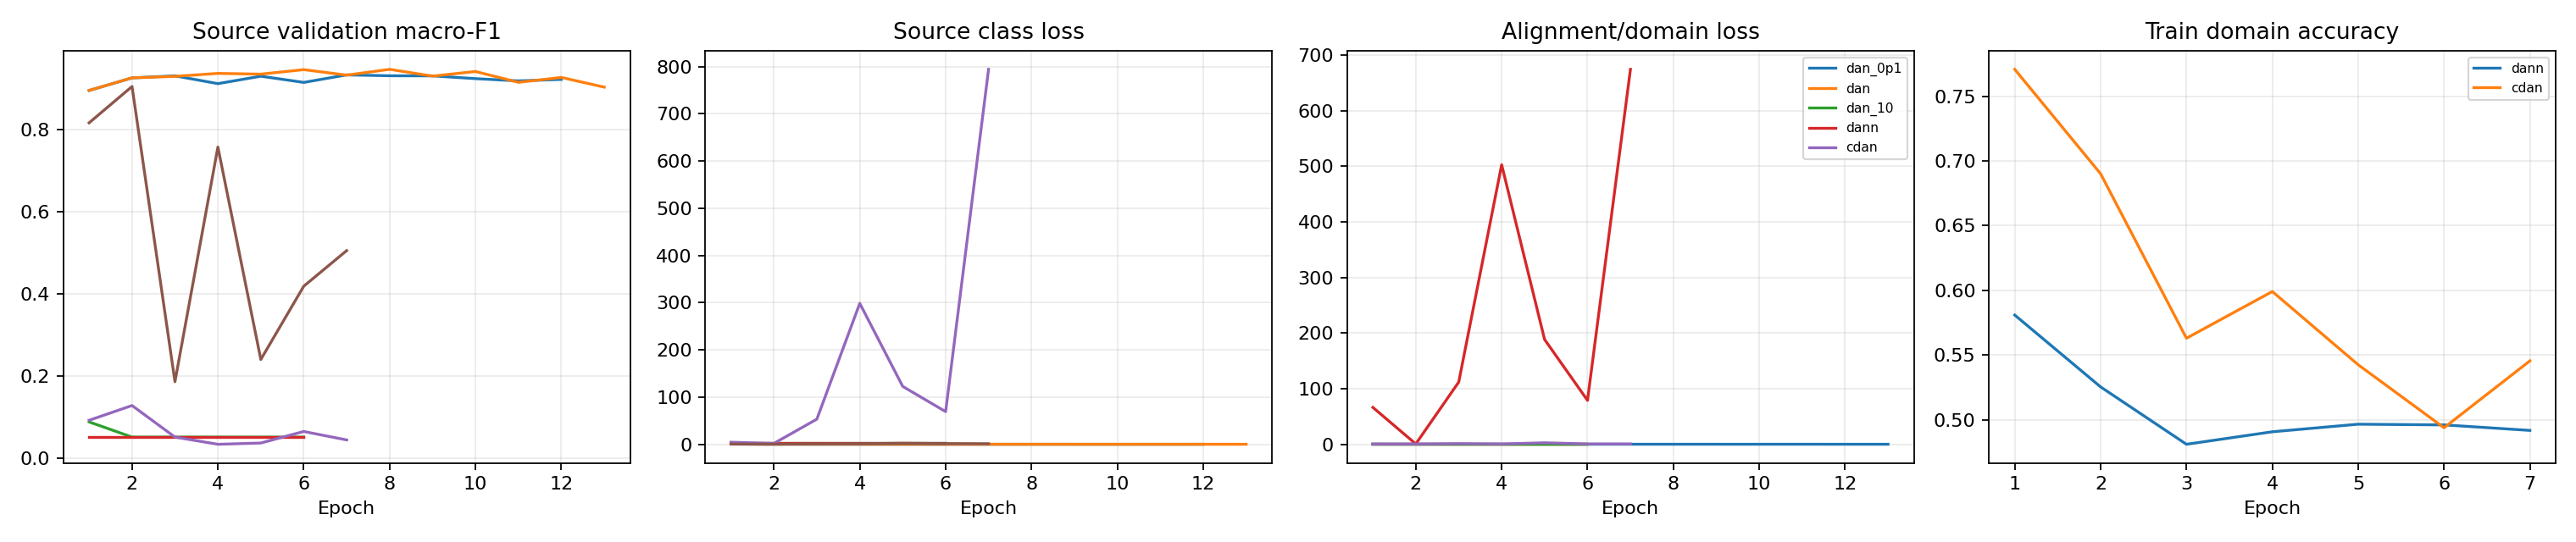
\includegraphics[width=\textwidth]{../task2/results/training_curves.png}
  \caption{Complete original Task 2 training curves for source-validation macro-F1, source classification loss, alignment/domain loss, and adversarial domain accuracy where applicable.}
\end{figure*}

\begin{table*}[h]
  \caption{Task 2 per-class Sketch accuracy. The final three rows are supplemental clipped runs.}
  \label{tab:t2-perclass}
  \centering
  \scriptsize
  \begin{tabular}{lrrrrrrr}
    \toprule
    Method & Dog & Elephant & Giraffe & Guitar & Horse & House & Person \\
    \midrule
    Source-only & 0.315 & 0.995 & 0.507 & 0.809 & 0.310 & 0.950 & 0.138 \\
    DAN 0.1 & 0.345 & 0.907 & 0.598 & 0.956 & 0.631 & 1.000 & 0.856 \\
    DAN 1 & 0.000 & 0.000 & 0.000 & 0.000 & 0.000 & 1.000 & 0.000 \\
    DAN 10 & 0.000 & 0.000 & 0.000 & 0.000 & 0.000 & 0.000 & 1.000 \\
    DANN & 0.000 & 0.004 & 0.000 & 0.000 & 0.000 & 0.388 & 0.775 \\
    CDAN & 0.291 & 0.001 & 0.158 & 0.870 & 0.315 & 1.000 & 1.000 \\
    \midrule
    DAN 1 + clip5 & 0.518 & 0.758 & 0.568 & 0.770 & 0.577 & 1.000 & 0.681 \\
    DANN + clip5 & 0.000 & 0.000 & 0.097 & 0.000 & 0.000 & 0.000 & 1.000 \\
    CDAN + clip5 & 0.692 & 0.191 & 0.684 & 0.964 & 0.854 & 1.000 & 0.806 \\
    \bottomrule
  \end{tabular}
\end{table*}

\begin{table}[h]
  \caption{Dominant failure pattern for unstable Task 2 methods.}
  \label{tab:t2-collapse}
  \centering
  \small
  \begin{tabular}{lll}
    \toprule
    Method & Dominant Sketch prediction & Evidence \\
    \midrule
    DAN 1 & House & 3,929/3,929 predictions \\
    DAN 10 & Person & 3,929/3,929 predictions \\
    DANN & House/person & Nearly all predictions \\
    DANN + clip5 & Person & Nearly all predictions \\
    \bottomrule
  \end{tabular}
\end{table}

\subsection{Supplemental clipped runs}
\begin{figure*}[h]
  \centering
  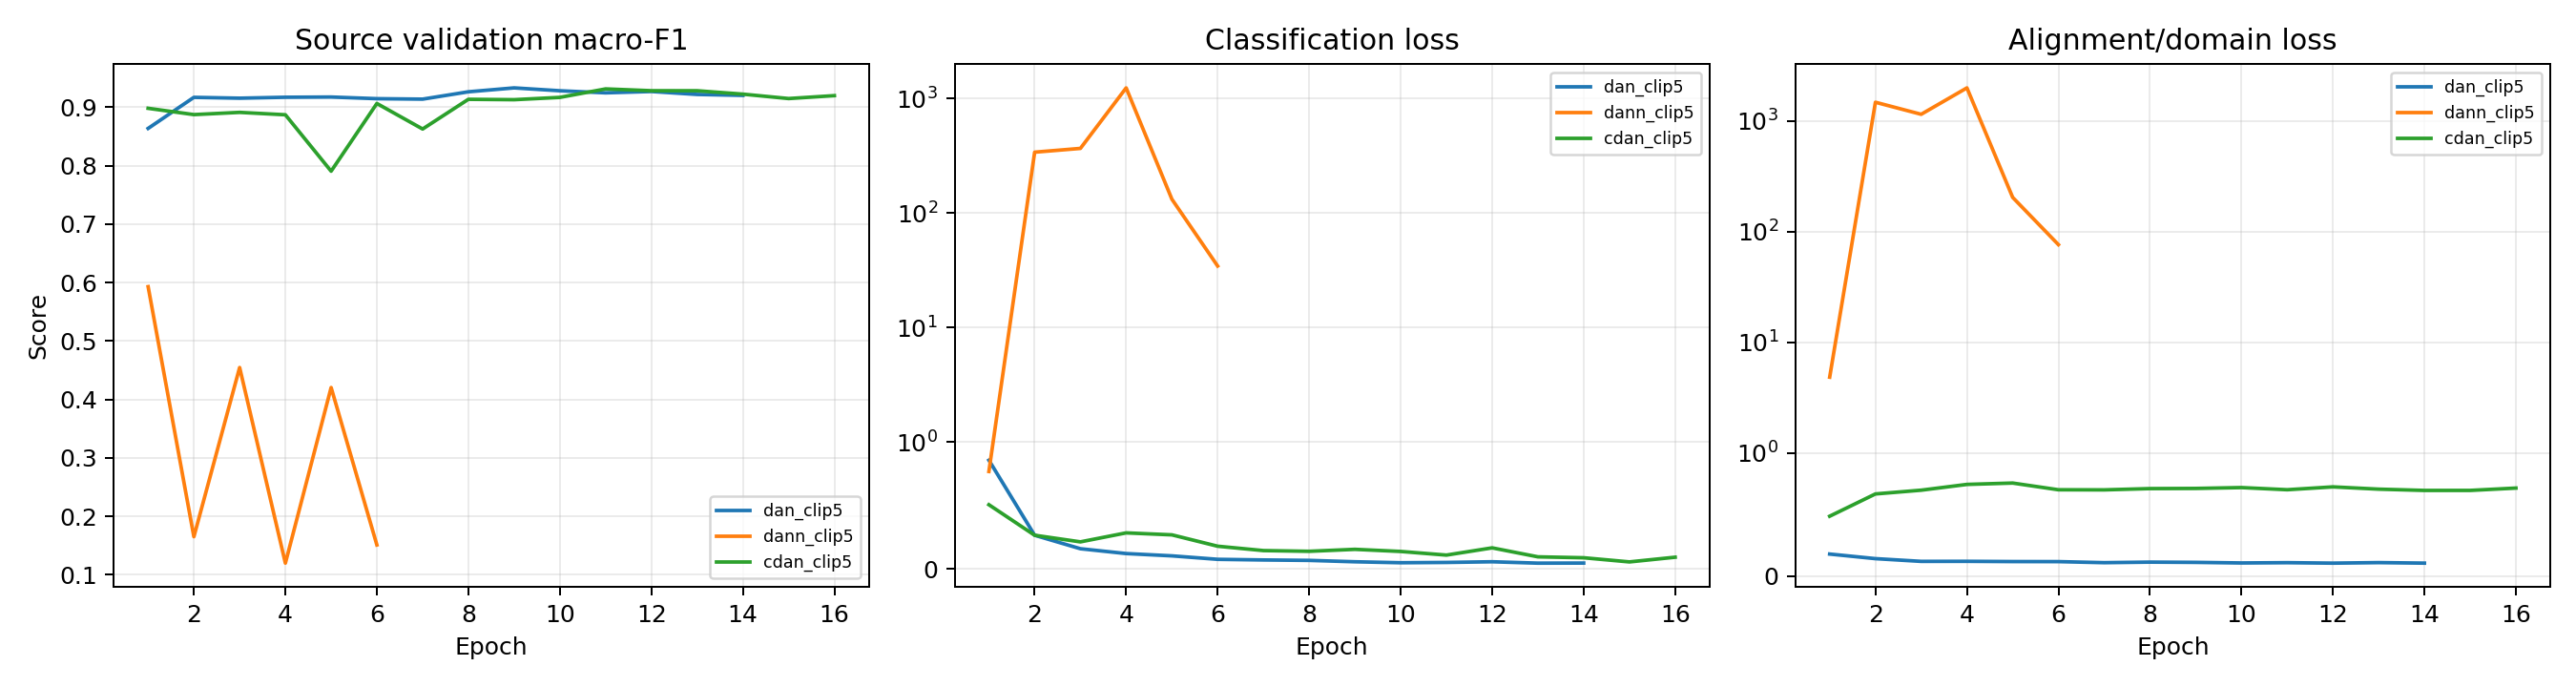
\includegraphics[width=\textwidth]{../task2/supplemental/results/training_curves.png}
  \caption{Complete supplemental Task 2 training curves after global gradient clipping at maximum norm 5; logarithmic loss axes expose both healthy and exploding trajectories.}
\end{figure*}

\begin{table*}[h]
  \caption{Complete supplemental Task 2 summary. Delta is Sketch accuracy relative to source-only ERM.}
  \label{tab:t2-supp-full}
  \centering
  \small
  \begin{tabular}{lrrrrrrr}
    \toprule
    Method & Epoch & Source acc. & Source F1 & Sketch acc. & Sketch F1 & Delta & Probe \\
    \midrule
    DAN 1 + clip5 & 9 & 0.9345 & 0.9331 & 0.6406 & 0.5982 & +0.0797 & 0.8214 \\
    DANN + clip5 & 1 & 0.6637 & 0.5929 & 0.0593 & 0.0363 & $-0.5017$ & 0.9986 \\
    CDAN + clip5 & 11 & 0.9301 & 0.9313 & 0.6826 & 0.6277 & +0.1217 & 0.9753 \\
    \bottomrule
  \end{tabular}
\end{table*}

\instruction{Discuss the supplemental rows in Tables~\ref{tab:t2-main} and \ref{tab:t2-perclass}. State that DANN still failed after clipping and that its epoch-mean pre-clip gradient norm reached 362,803.}

\clearpage
\section{Task 3 supporting results}
\label{app:t3}

\subsection{Original curves and diagnostics}
\begin{figure*}[h]
  \centering
  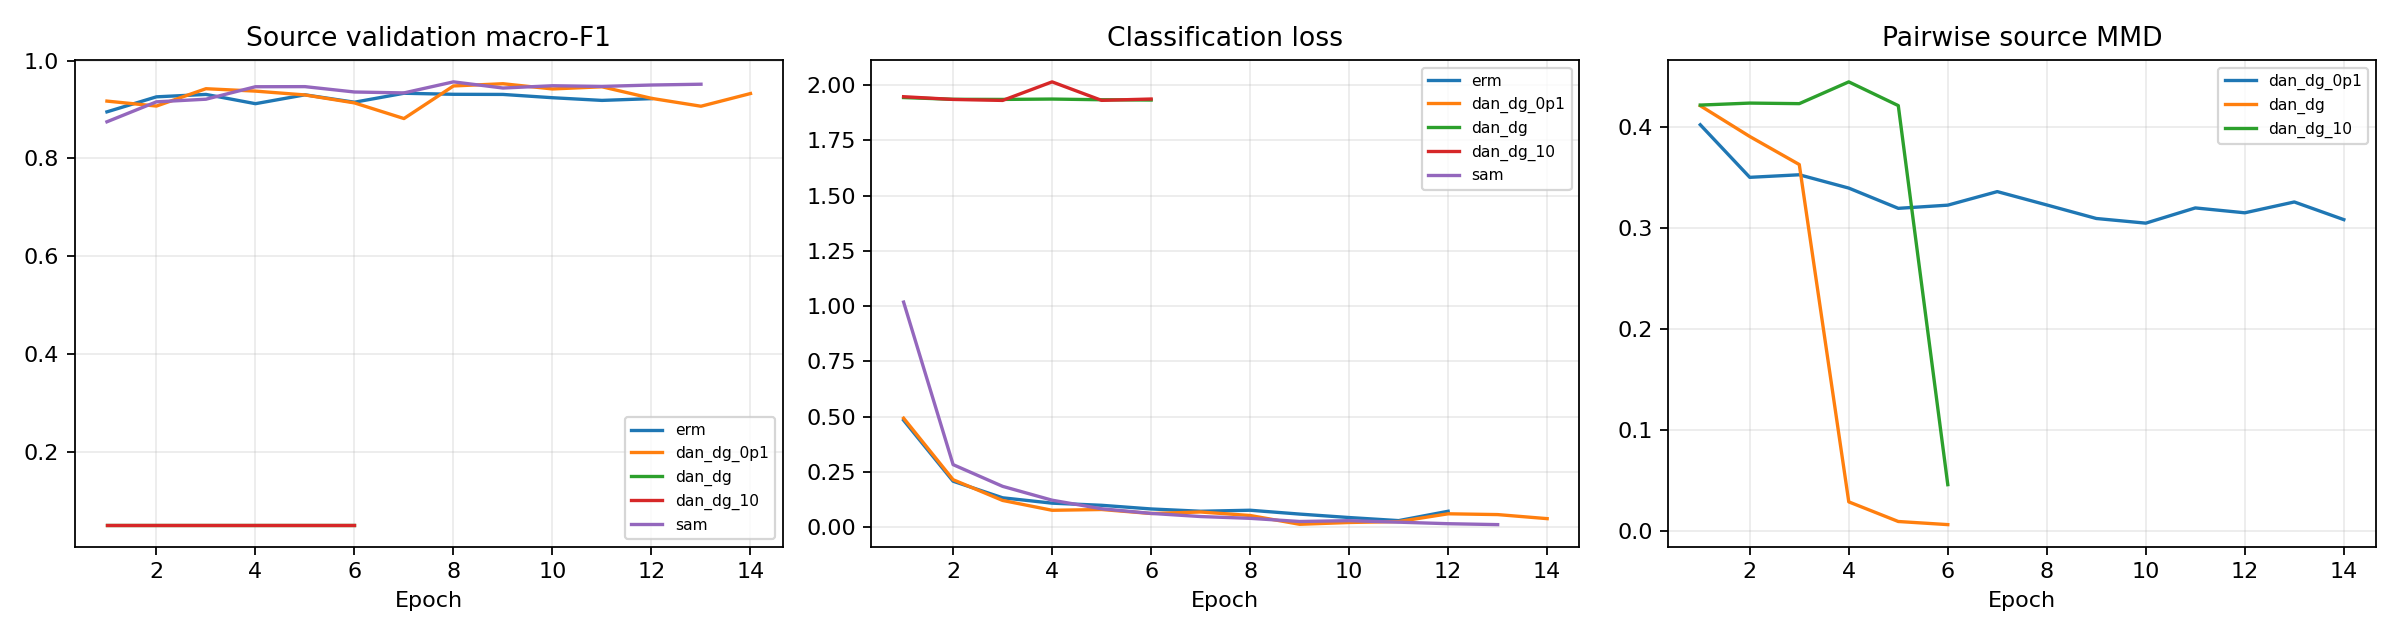
\includegraphics[width=\textwidth]{../task3/results/training_curves.png}
  \caption{Original Task 3 source-validation macro-F1 and objective trajectories, including the one-class failures for DAN-DG $\lambda=1$ and $10$.}
\end{figure*}

\begin{table*}[h]
  \caption{Task 3 per-class Sketch accuracy. The final two rows are supplemental stabilization runs.}
  \label{tab:t3-perclass}
  \centering
  \scriptsize
  \begin{tabular}{lrrrrrrr}
    \toprule
    Method & Dog & Elephant & Giraffe & Guitar & Horse & House & Person \\
    \midrule
    ERM & 0.315 & 0.995 & 0.507 & 0.809 & 0.310 & 0.950 & 0.138 \\
    DAN-DG 0.1 & 0.494 & 0.858 & 0.710 & 0.910 & 0.582 & 0.825 & 0.925 \\
    DAN-DG 1 & 0.000 & 0.000 & 0.000 & 0.000 & 0.000 & 0.000 & 1.000 \\
    DAN-DG 10 & 0.000 & 0.000 & 0.000 & 0.000 & 0.000 & 0.000 & 1.000 \\
    SAM & 0.503 & 0.958 & 0.645 & 0.885 & 0.559 & 0.912 & 0.738 \\
    \midrule
    DAN-DG 1 + clip5 & 0.000 & 0.000 & 0.000 & 0.000 & 0.000 & 0.000 & 1.000 \\
    DAN-DG 1 norm + clip5 & 0.163 & 0.977 & 0.798 & 0.789 & 0.449 & 0.975 & 0.537 \\
    \bottomrule
  \end{tabular}
\end{table*}

\begin{table*}[h]
  \caption{Task 3 source-domain validation results. The worst domain is Art Painting for every healthy original model and Cartoon for the collapsed DAN-DG models.}
  \label{tab:t3-source}
  \centering
  \scriptsize
  \begin{tabular}{lrrrrrrrr}
    \toprule
    Method & Photo acc. & Photo F1 & Art acc. & Art F1 & Cartoon acc. & Cartoon F1 & Mean acc. & Mean F1 \\
    \midrule
    ERM & 0.9731 & 0.9693 & 0.9073 & 0.8995 & 0.9275 & 0.9314 & 0.9360 & 0.9334 \\
    DAN-DG 0.1 & 0.9701 & 0.9663 & 0.9244 & 0.9249 & 0.9638 & 0.9675 & 0.9527 & 0.9529 \\
    DAN-DG 1 & 0.2575 & 0.0585 & 0.2195 & 0.0514 & 0.1727 & 0.0421 & 0.2166 & 0.0507 \\
    DAN-DG 10 & 0.2575 & 0.0585 & 0.2195 & 0.0514 & 0.1727 & 0.0421 & 0.2166 & 0.0507 \\
    SAM & 0.9701 & 0.9647 & 0.9390 & 0.9394 & 0.9616 & 0.9659 & 0.9569 & 0.9567 \\
    \bottomrule
  \end{tabular}
\end{table*}

\instruction{Use Tables~\ref{tab:t3-perclass} and \ref{tab:t3-source} when discussing per-source performance, collapse, and class balance. Explain the balanced three-way linear separability diagnostic and the fixed-radius sharpness protocol in prose.}

\subsection{Task 2 versus Task 3}
\begin{table*}[h]
  \caption{Target-aware versus target-free transfer. Prescribed $\lambda=1$ rows are shown separately from the successful $\lambda=0.1$ sensitivity runs.}
  \label{tab:t2-t3-comparison}
  \centering
  \small
  \begin{tabular}{lllrr}
    \toprule
    Status & Method & Target access & Sketch acc. & Sketch F1 \\
    \midrule
    Baseline & ERM & None & 0.5610 & 0.5745 \\
    Prescribed & Task 2 DAN 1 & Unlabeled Sketch & 0.0204 & 0.0057 \\
    Prescribed & Task 3 DAN-DG 1 & No Sketch & 0.0407 & 0.0112 \\
    Sensitivity & Task 2 DAN 0.1 & Unlabeled Sketch & 0.6872 & 0.6349 \\
    Sensitivity & Task 3 DAN-DG 0.1 & No Sketch & \textbf{0.7109} & 0.7199 \\
    Original & Task 3 SAM & No Sketch & 0.7045 & \textbf{0.7466} \\
    \bottomrule
  \end{tabular}
\end{table*}

\subsection{Supplemental fallback sequence}
\begin{table*}[h]
  \caption{Supplemental DAN-DG $\lambda=1$ fallback sequence.}
  \centering
  \scriptsize
  \begin{tabular}{lrrrrrrrr}
    \toprule
    Variant & Source acc. & Source F1 & Worst acc. & Worst F1 & Sketch acc. & Sketch F1 & Separability & Sharpness \\
    \midrule
    Original & 0.2166 & 0.0507 & 0.1727 & 0.0421 & 0.0407 & 0.0112 & 0.5847 & 0.0103 \\
    Clip5 & 0.2166 & 0.0507 & 0.1727 & 0.0421 & 0.0407 & 0.0112 & 0.5914 & 0.0088 \\
    Normalized MMD + clip5 & 0.9304 & 0.9284 & 0.9000 & 0.8959 & 0.6261 & 0.6321 & 0.6611 & 46.9051 \\
    \bottomrule
  \end{tabular}
\end{table*}

\begin{figure*}[h]
  \centering
  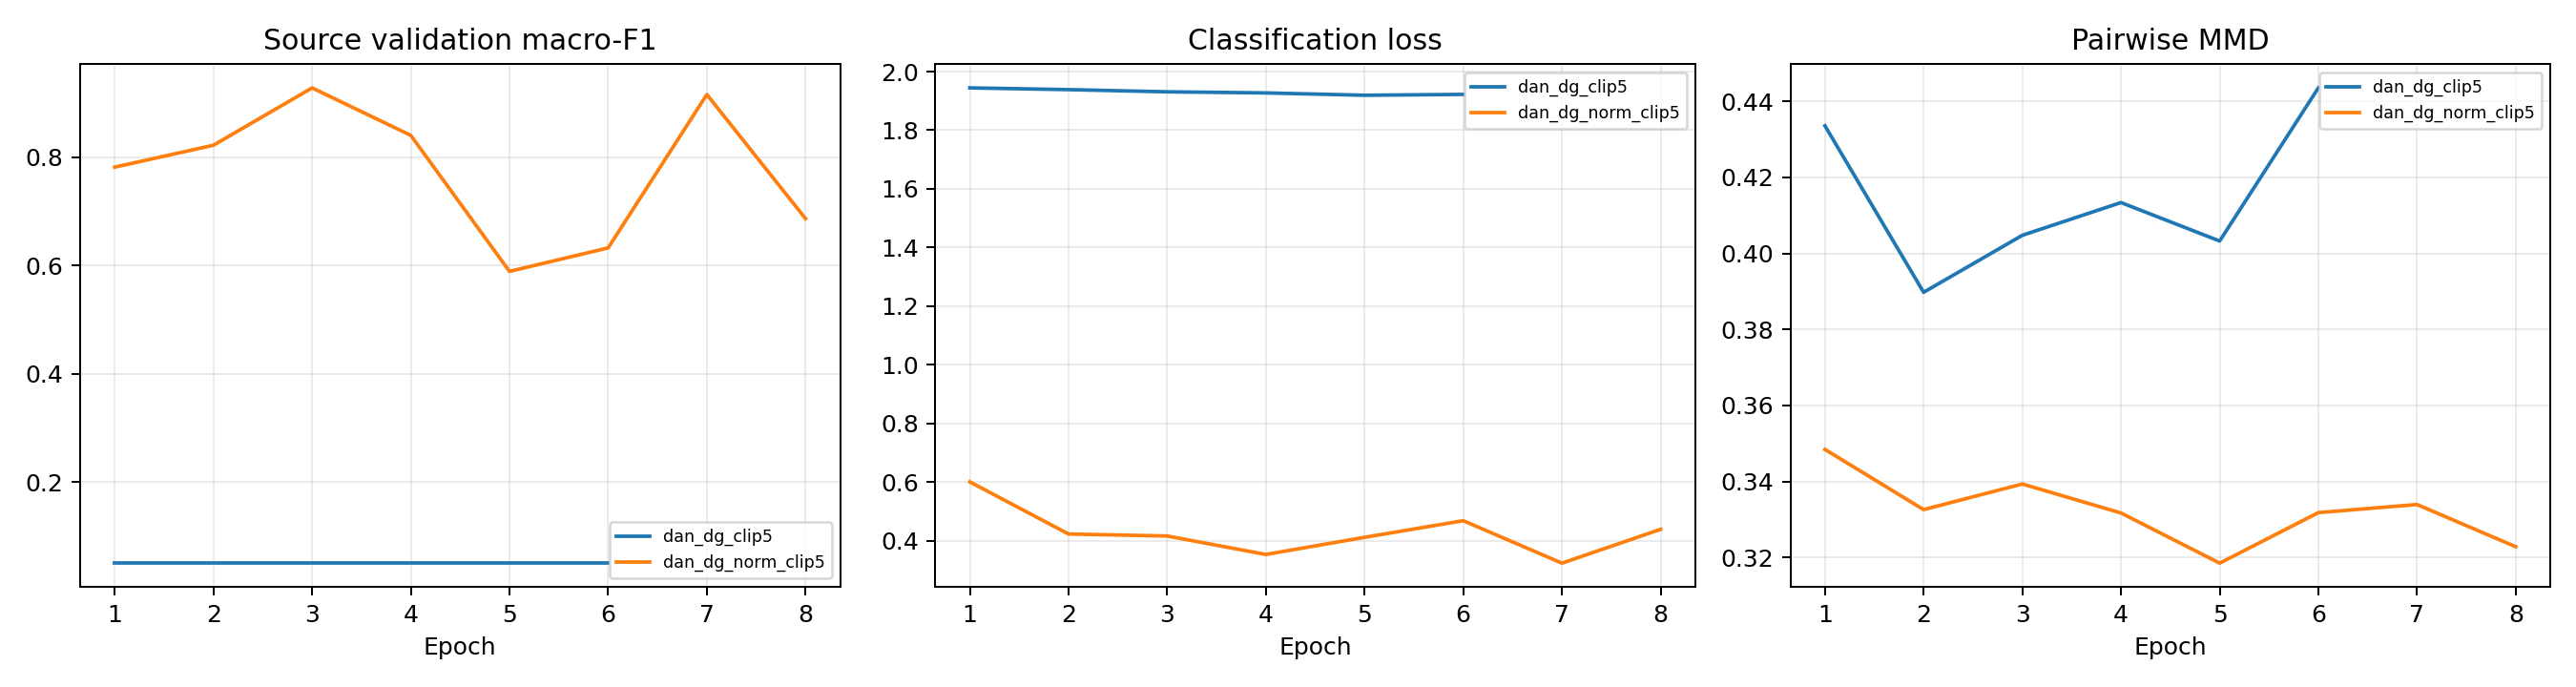
\includegraphics[width=\textwidth]{../task3/supplemental/results/training_curves.png}
  \caption{Supplemental Task 3 trajectories for clipping alone and the normalized-MMD-plus-clipping fallback. Selection remained source-only.}
\end{figure*}

\instruction{Explain the source-only fallback gate, deterioration after epoch 3, and sharpness 46.9051. Do not call the recovered variant flat.}

\clearpage
\section{Task 4 supporting results}
\label{app:t4}

\subsection{Data protocol and known-class training}
\begin{table}[h]
  \caption{CIFAR data protocol. CIFAR-100 subsets are used only for final unknown evaluation.}
  \label{tab:t4-data}
  \centering
  \small
  \begin{tabular}{llr}
    \toprule
    Data & Use & Count \\
    \midrule
    CIFAR-10 train & Optimization & 45,000 \\
    CIFAR-10 validation & Selection/thresholds & 5,000 \\
    CIFAR-10 test & Final known evaluation & 10,000 \\
    CIFAR-100 Near & Unknown evaluation & 800 \\
    CIFAR-100 Far & Unknown evaluation & 800 \\
    \bottomrule
  \end{tabular}
\end{table}

\instruction{State the exact unknown classes: Near = bus, pickup truck, motorcycle, tractor, wolf, fox, leopard, camel; Far = bottle, bowl, chair, clock, keyboard, mushroom, sunflower, wardrobe. Describe the complete model settings in prose.}

\begin{table}[h]
  \caption{CIFAR-10 known-class performance.}
  \centering
  \small
  \begin{tabular}{lrrrr}
    \toprule
    Model & Selected epoch & Best val. (\%) & Final val. (\%) & Test (\%) \\
    \midrule
    Vanilla & 100 & 94.82 & 94.82 & 94.67 \\
    GCSC & 99 & 95.32 & 95.30 & \textbf{95.35} \\
    PROSER & 1 & 94.38 & 82.62 & 94.07 \\
    \bottomrule
  \end{tabular}
\end{table}

\instruction{Explain healthy Vanilla/GCSC training, GCSC's 0.68-point test improvement, PROSER's deteriorating trajectory, and best-checkpoint protection. Call the trajectory unstable; do not call the selected epoch-1 checkpoint collapsed.}

\subsection{Complete score and failure analysis}
\begin{table*}[h]
  \caption{Complete original and supplemental open-set metrics. Thresholds are selected from CIFAR-10 validation only. FPR is the accepted-unknown fraction and equals one minus unknown rejection.}
  \label{tab:t4-full-osr}
  \centering
  \scriptsize
  \begin{tabular}{lllrrrrr}
    \toprule
    Model & Score & Group & Threshold & AUROC & Known accept. & Unknown reject. & FPR \\
    \midrule
    Vanilla & MSP & Near & 0.1627 & 0.8265 & 0.9500 & 0.2900 & 0.7100 \\
    Vanilla & MSP & Far & 0.1627 & 0.9061 & 0.9500 & 0.4638 & 0.5363 \\
    Vanilla & MSP & All & 0.1627 & 0.8663 & 0.9500 & 0.3769 & 0.6231 \\
    Vanilla & MLS & Near & $-5.826$ & 0.8117 & 0.9466 & 0.3563 & 0.6438 \\
    Vanilla & MLS & Far & $-5.826$ & 0.9075 & 0.9466 & 0.5775 & 0.4225 \\
    Vanilla & MLS & All & $-5.826$ & 0.8596 & 0.9466 & 0.4669 & 0.5331 \\
    Vanilla & Energy & Near & $-6.043$ & 0.8117 & 0.9444 & 0.3663 & 0.6338 \\
    Vanilla & Energy & Far & $-6.043$ & 0.9081 & 0.9444 & 0.5875 & 0.4125 \\
    Vanilla & Energy & All & $-6.043$ & 0.8599 & 0.9444 & 0.4769 & 0.5231 \\
    Vanilla & Mahalanobis & Near & 2906.45 & 0.8007 & 0.9523 & 0.2675 & 0.7325 \\
    Vanilla & Mahalanobis & Far & 2906.45 & 0.9201 & 0.9523 & 0.5275 & 0.4725 \\
    Vanilla & Mahalanobis & All & 2906.45 & 0.8604 & 0.9523 & 0.3975 & 0.6025 \\
    GCSC & MLS & Near & $-6.040$ & 0.8076 & 0.9494 & 0.3300 & 0.6700 \\
    GCSC & MLS & Far & $-6.040$ & 0.9078 & 0.9494 & 0.5775 & 0.4225 \\
    GCSC & MLS & All & $-6.040$ & 0.8577 & 0.9494 & 0.4538 & 0.5463 \\
    PROSER & MLS & Near & $-4.470$ & 0.8117 & 0.9480 & 0.3125 & 0.6875 \\
    PROSER & MLS & Far & $-4.470$ & 0.8708 & 0.9480 & 0.4550 & 0.5450 \\
    PROSER & MLS & All & $-4.470$ & 0.8413 & 0.9480 & 0.3838 & 0.6163 \\
    PROSER & Placeholder & Near & $5.877\!\times\!10^{-5}$ & 0.8067 & 0.9484 & 0.3138 & 0.6863 \\
    PROSER & Placeholder & Far & $5.877\!\times\!10^{-5}$ & 0.8927 & 0.9484 & 0.5213 & 0.4788 \\
    PROSER & Placeholder & All & $5.877\!\times\!10^{-5}$ & 0.8497 & 0.9484 & 0.4175 & 0.5825 \\
    \midrule
    PROSER clip5 & MLS & Near & $-4.486$ & 0.8123 & 0.9471 & 0.3150 & 0.6850 \\
    PROSER clip5 & MLS & Far & $-4.486$ & 0.8704 & 0.9471 & 0.4550 & 0.5450 \\
    PROSER clip5 & MLS & All & $-4.486$ & 0.8414 & 0.9471 & 0.3850 & 0.6150 \\
    PROSER clip5 & Placeholder & Near & $5.941\!\times\!10^{-5}$ & 0.8076 & 0.9490 & 0.3150 & 0.6850 \\
    PROSER clip5 & Placeholder & Far & $5.941\!\times\!10^{-5}$ & 0.8926 & 0.9490 & 0.5213 & 0.4788 \\
    PROSER clip5 & Placeholder & All & $5.941\!\times\!10^{-5}$ & 0.8501 & 0.9490 & 0.4181 & 0.5819 \\
    \bottomrule
  \end{tabular}
\end{table*}

\begin{figure*}[h]
  \centering
  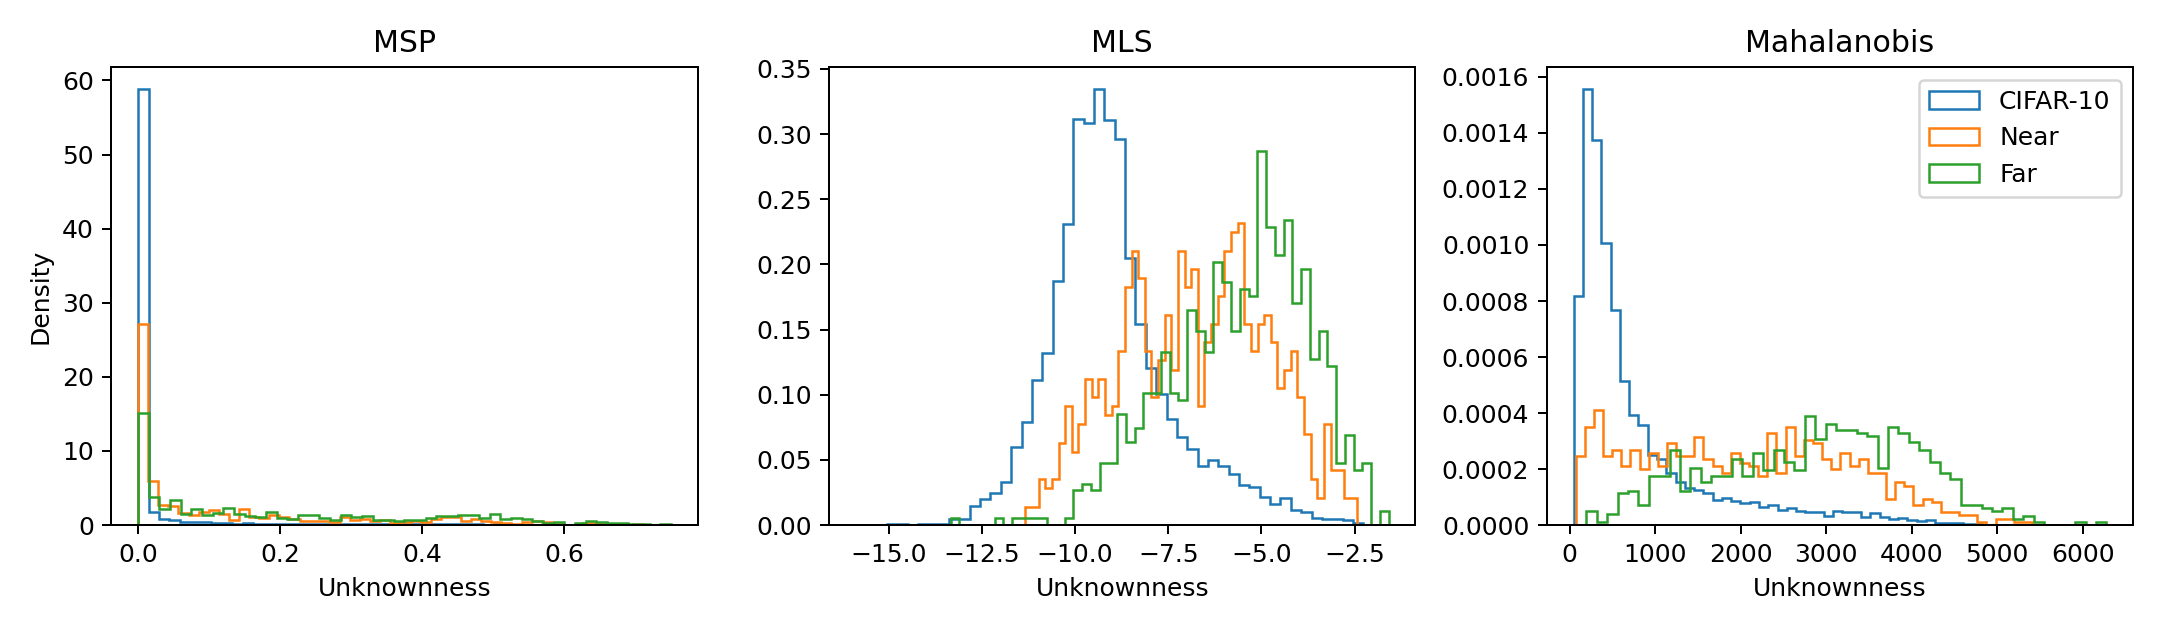
\includegraphics[width=\textwidth]{../task4/results/vanilla_score_distributions.png}
  \caption{Vanilla CIFAR-10, Near, and Far unknownness distributions for MSP, MLS, and Mahalanobis scores. Larger values indicate greater unknownness.}
\end{figure*}

\begin{table*}[h]
  \caption{Selected high-confidence Vanilla MLS failures shown in the failure gallery. Scores below the validation threshold are incorrectly accepted as known.}
  \label{tab:t4-failures}
  \centering
  \small
  \begin{tabular}{llrlrrl}
    \toprule
    Group & Unknown class & CIFAR-100 index & Predicted class & MLS score & Threshold & Classification \\
    \midrule
    Near & Bus & 4296 & Truck & $-11.333$ & $-5.826$ & Plausible \\
    Near & Bus & 6116 & Truck & $-11.279$ & $-5.826$ & Plausible \\
    Near & Bus & 8655 & Truck & $-11.128$ & $-5.826$ & Plausible \\
    Far & Keyboard & 6297 & Bird & $-13.336$ & $-5.826$ & Surprising \\
    Far & Sunflower & 5260 & Bird & $-12.013$ & $-5.826$ & Surprising \\
    Far & Mushroom & 8701 & Dog & $-11.469$ & $-5.826$ & Surprising \\
    \bottomrule
  \end{tabular}
\end{table*}

\begin{figure*}[h]
  \centering
  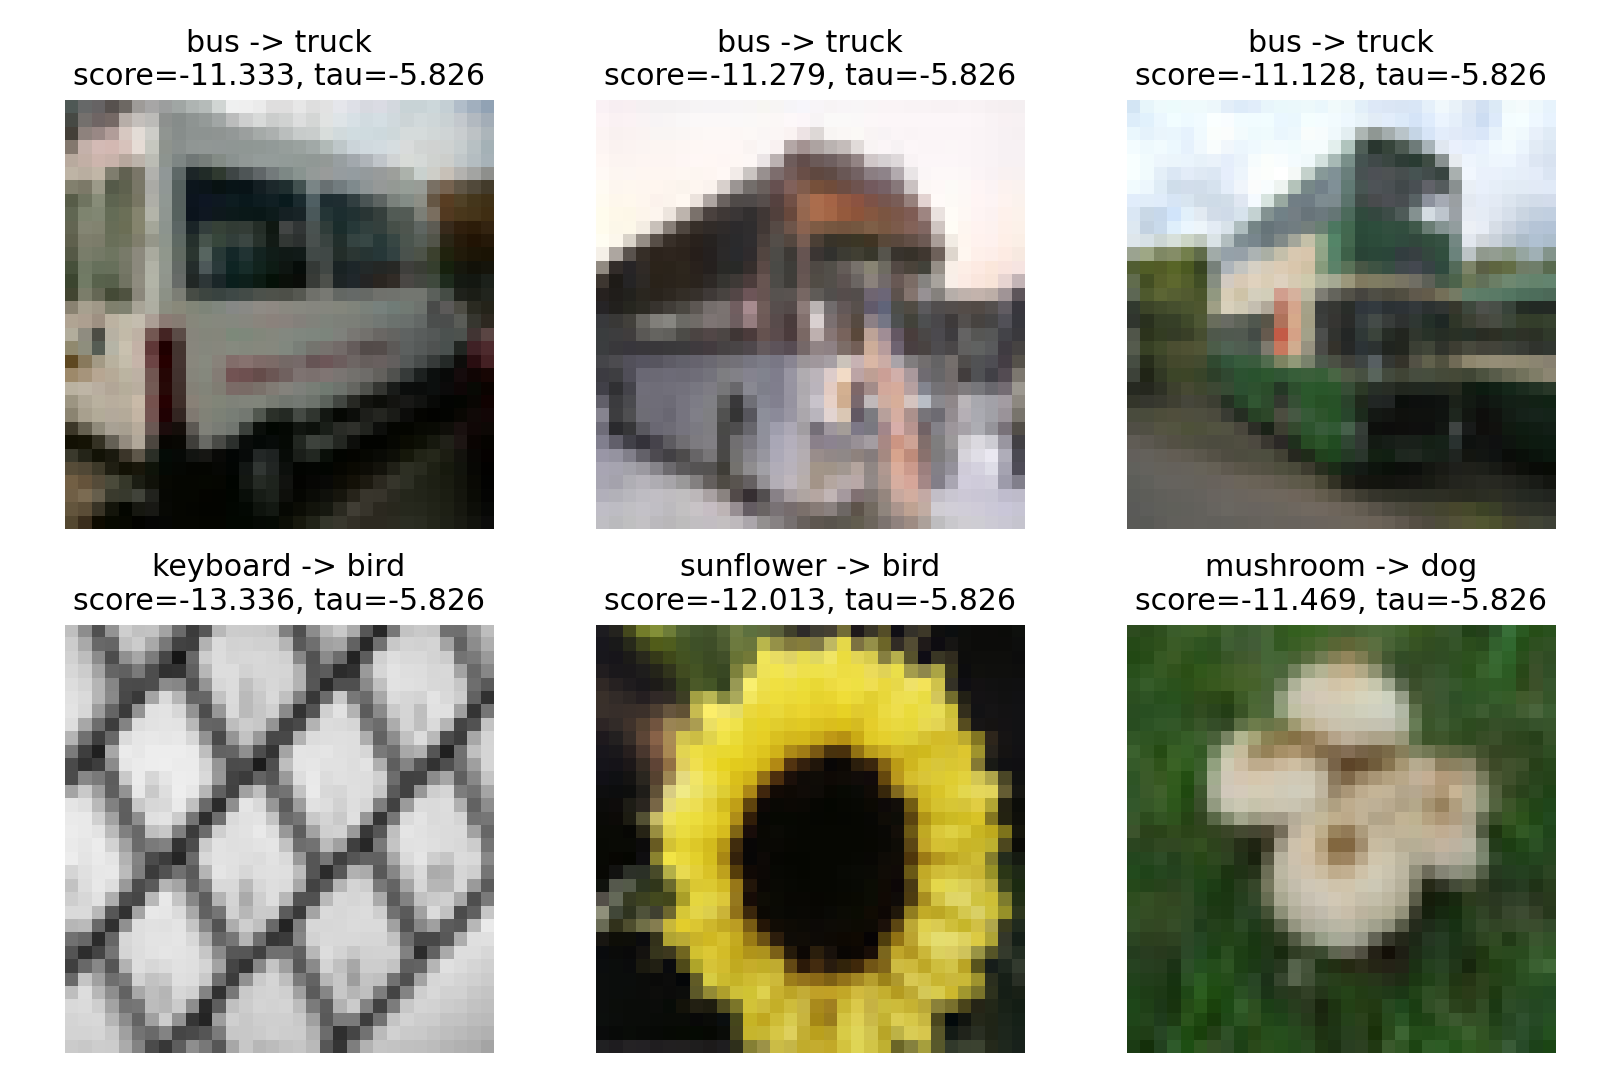
\includegraphics[width=\textwidth]{../task4/results/vanilla_mls_failures.png}
  \caption{High-confidence Vanilla MLS failures beyond the validation threshold. The top row contains Near bus-to-truck errors; the bottom row contains semantically Far errors.}
\end{figure*}

\subsection{Supplemental PROSER clipping}
\begin{table}[h]
  \caption{Original versus clipped PROSER.}
  \centering
  \small
  \begin{tabular}{lrrr}
    \toprule
    Quantity & Original & Clip5 & Change \\
    \midrule
    Best validation acc. & 0.9438 & 0.9446 & +0.0008 \\
    Epoch-50 validation acc. & 0.8262 & 0.9040 & +0.0778 \\
    Test acc. & 0.9407 & 0.9408 & +0.0001 \\
    MLS All AUROC & 0.8413 & 0.8414 & +0.0001 \\
    Placeholder All AUROC & 0.8497 & 0.8501 & +0.0003 \\
    Placeholder All rejection & 0.4175 & 0.4181 & +0.0006 \\
    \bottomrule
  \end{tabular}
\end{table}

\begin{table*}[h]
  \caption{PROSER validation trajectories and supplemental diagnostics. Dummy-win rate and pre-clip gradient norm were added in the clipped run.}
  \label{tab:t4-proser-trajectory}
  \centering
  \small
  \begin{tabular}{rrrrr}
    \toprule
    Epoch & Original val. acc. & Clip5 val. acc. & Clip5 dummy-win rate & Clip5 grad. norm \\
    \midrule
    1 & 0.9438 & 0.9446 & 0.0802 & 2.5665 \\
    10 & 0.9348 & 0.9352 & 0.8142 & 4.6787 \\
    20 & 0.9184 & 0.9258 & 0.9996 & 2.1767 \\
    30 & 0.7910 & 0.8986 & 1.0000 & 1.6980 \\
    40 & 0.8304 & 0.8946 & 1.0000 & 1.1246 \\
    50 & 0.8262 & 0.9040 & 1.0000 & 1.2263 \\
    \bottomrule
  \end{tabular}
\end{table*}

\instruction{Use Table~\ref{tab:t4-proser-trajectory} to explain that clipping improves late validation behavior but barely changes selected-checkpoint OSR. The recorded epoch-mean pre-clip gradient norms range from 1.1246 to 4.6787.}

\clearpage
\section{Reproducibility inventory}
\instruction{Optionally list artifact filenames, checkpoint hashes, commands/configuration files, software versions, hardware, and seed 6304. Include useful reproducibility information rather than raw logs.}

\section{Final author checklist}
\begin{itemize}
  \item \textbf{[Replace or delete every blue bracketed instruction.]}
  \item \textbf{[Replace the placeholder title and author fields; revise factual captions only if needed.]}
  \item \textbf{[Confirm every included image renders at readable size.]}
  \item \textbf{[Ensure the main conclusion ends on or before page 12.]}
  \item \textbf{[Do not modify \texttt{neurips\_2026.sty} to save space.]}
  \item \textbf{[Cite every table, figure, and appendix section from the prose.]}
  \item \textbf{[Label every supplemental row and disclose clipping/normalization.]}
  \item \textbf{[Use percentage points for differences between accuracies.]}
  \item \textbf{[Discuss cue shape bias together with coverage.]}
  \item \textbf{[Never praise collapsed runs for low separability or sharpness.]}
  \item \textbf{[Retain the normalized DAN-DG sharpness caveat.]}
  \item \textbf{[Distinguish selected PROSER from its unstable later trajectory.]}
  \item \textbf{[State target/unknown isolation for Tasks 2--4.]}
  \item \textbf{[Do not generalize beyond the single-seed/domain setup.]}
  \item \textbf{[Check the final PDF at 100\% zoom for cropped tables and unreadable panels.]}
\end{itemize}

\end{document}
